\documentclass[12pt]{article}
\usepackage{amsmath, amssymb, amsthm}
\usepackage{mathtools}
\usepackage{graphicx}
\usepackage{float}
\usepackage{hyperref}
\usepackage{xcolor}
\usepackage{listings}
\usepackage{geometry}
\usepackage{algorithm}
\usepackage{algpseudocode}
\usepackage{tikz}
\usepackage{longtable}
\usepackage{circuitikz}
\usepackage{comment}
\usepackage{MnSymbol}
\usepackage{physics}
\usepackage[section]{placeins}
\usepackage{subfig}
\geometry{a4paper, margin=1in}

\title{Comparison of Numerical Methods with Fourier Series Solution}
\author{}
\date{}

\begin{document}

\maketitle

\tableofcontents
\newpage

\section{Introduction}
This report presents a visual comparison between various numerical methods and the Fourier series solution for an RL circuit with a PWM input. The numerical methods compared are:
\begin{itemize}
    \item Euler Method
    \item RK2 Method (2nd order Runge-Kutta)
    \item RK4 Method (4th order Runge-Kutta)
    \item Reverse Euler Method
    \item Trapezoidal Method
\end{itemize}

\section{Parameter Configurations}
The comparisons are made across different parameter configurations:
\begin{itemize}
    \item Resistance (R): 1000 $\Omega$, 100 $\Omega$, 1 $\Omega$, 0.001 $\Omega$
    \item Inductance (L): 1 H
    \item Time step (h): T/10, T/1000 (where T = 0.1s is the time period)
    \item Duty cycle ($\alpha$): 0.4
    \item Amplitude (A): 10.0
\end{itemize}

\section{Results for R = 1000 $\Omega$}

\subsection{Time Step h = T/10}

\begin{figure}[H]
    \centering
    \subfloat[Fourier vs Euler]{
        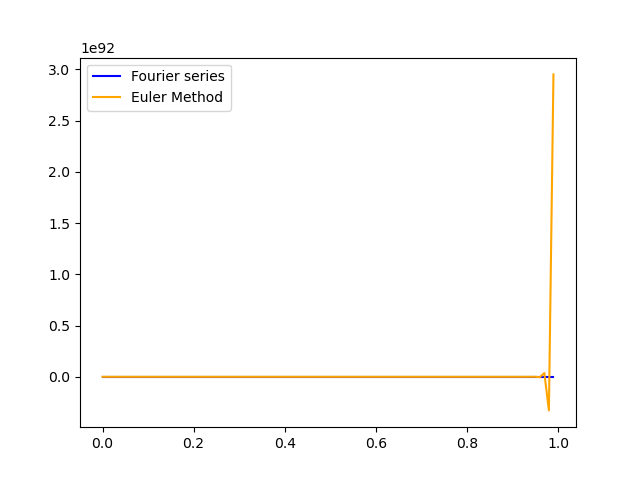
\includegraphics[width=0.45\textwidth]{figs/euler_R1000_L1_h0.01.png}
    }
    \subfloat[Euler Error]{
        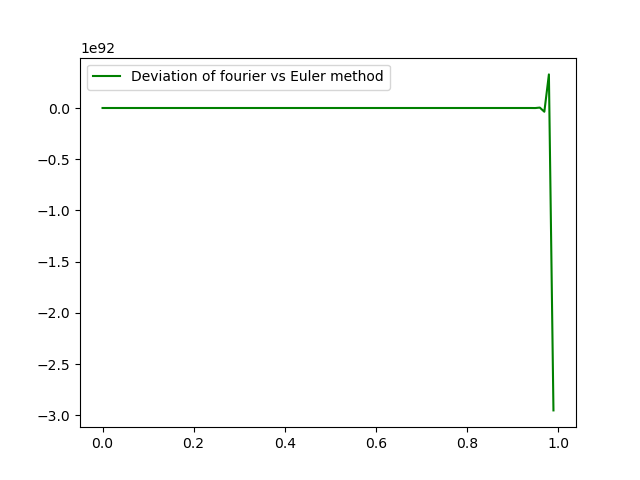
\includegraphics[width=0.45\textwidth]{figs/eulerError_R1000_L1_h0.01.png}
    }
    \caption{Euler Method Comparison (R = 1000 $\Omega$, L = 1 H, h = T/10)}
\end{figure}

\begin{figure}[H]
    \centering
    \subfloat[Fourier vs RK2]{
        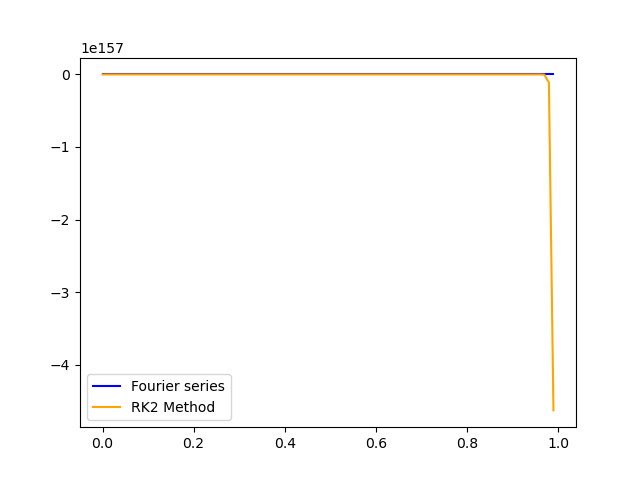
\includegraphics[width=0.45\textwidth]{figs/rk2_R1000_L1_h0.01.png}
    }
    \subfloat[RK2 Error]{
        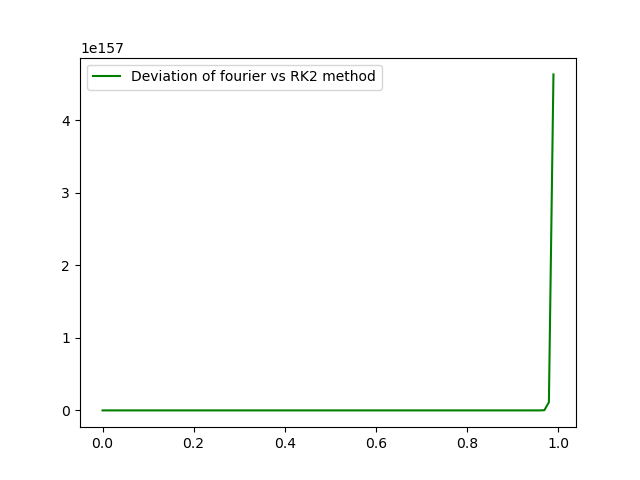
\includegraphics[width=0.45\textwidth]{figs/rk2Error_R1000_L1_h0.01.png}
    }
    \caption{RK2 Method Comparison (R = 1000 $\Omega$, L = 1 H, h = T/10)}
\end{figure}

\begin{figure}[H]
    \centering
    \subfloat[Fourier vs RK4]{
        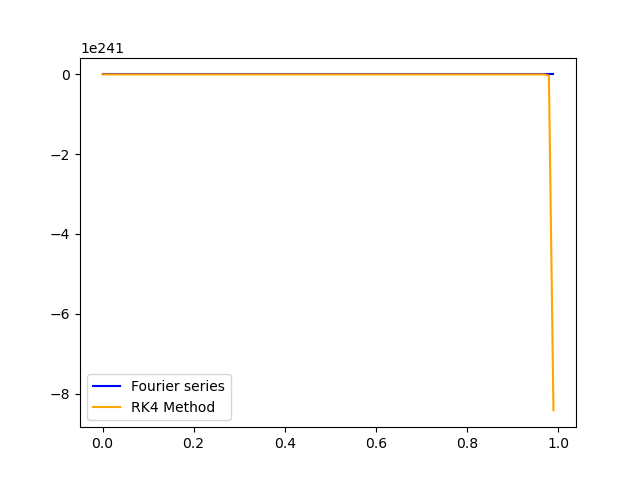
\includegraphics[width=0.45\textwidth]{figs/rk4_R1000_L1_h0.01.png}
    }
    \subfloat[RK4 Error]{
        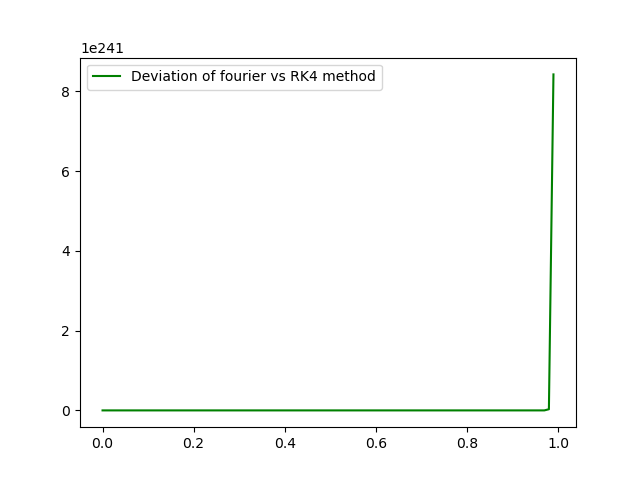
\includegraphics[width=0.45\textwidth]{figs/rk4Error_R1000_L1_h0.01.png}
    }
    \caption{RK4 Method Comparison (R = 1000 $\Omega$, L = 1 H, h = T/10)}
\end{figure}

\begin{figure}[H]
    \centering
    \subfloat[Fourier vs Reverse Euler]{
        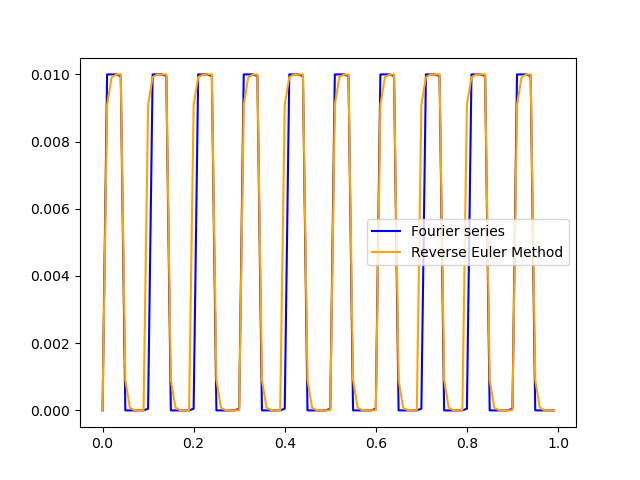
\includegraphics[width=0.45\textwidth]{figs/reverseEuler_R1000_L1_h0.01.png}
    }
    \subfloat[Reverse Euler Error]{
        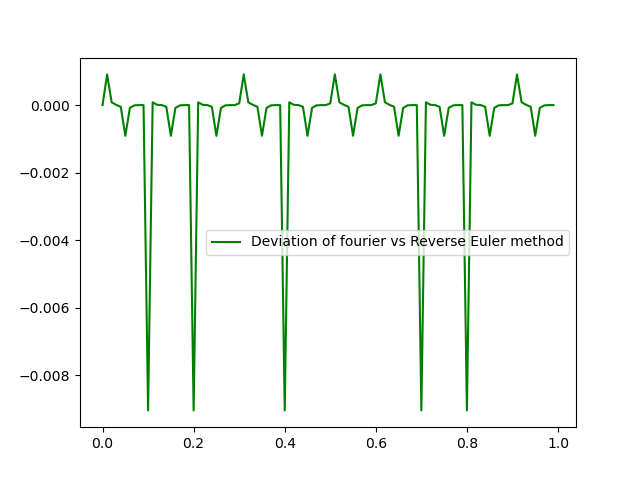
\includegraphics[width=0.45\textwidth]{figs/reverseEulerError_R1000_L1_h0.01.png}
    }
    \caption{Reverse Euler Method Comparison (R = 1000 $\Omega$, L = 1 H, h = T/10)}
\end{figure}

\begin{figure}[H]
    \centering
    \subfloat[Fourier vs Trapezoidal]{
        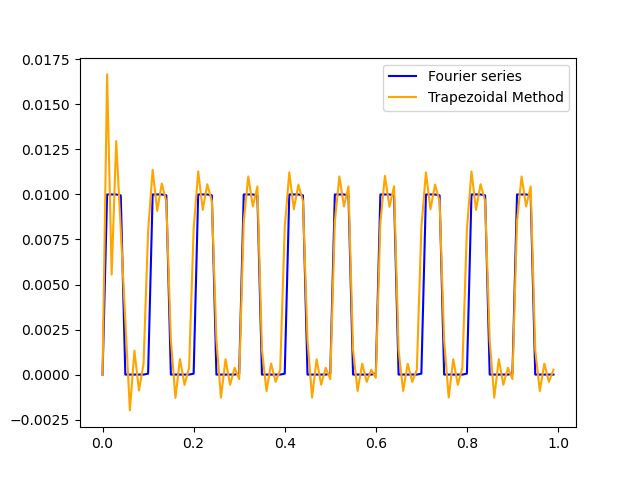
\includegraphics[width=0.45\textwidth]{figs/trapezoidal_R1000_L1_h0.01.png}
    }
    \subfloat[Trapezoidal Error]{
        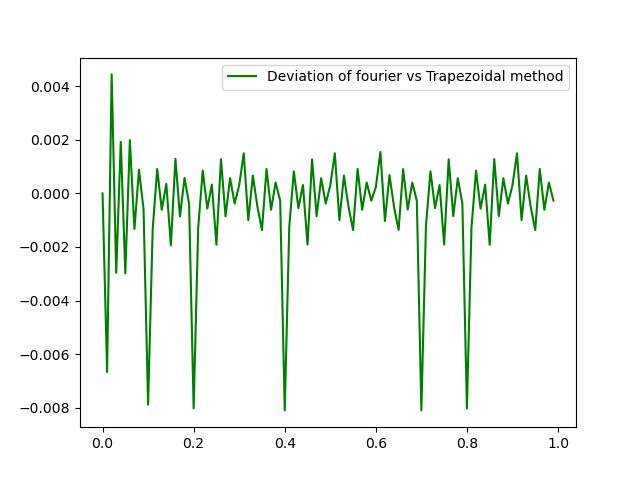
\includegraphics[width=0.45\textwidth]{figs/trapezoidalError_R1000_L1_h0.01.png}
    }
    \caption{Trapezoidal Method Comparison (R = 1000 $\Omega$, L = 1 H, h = T/10)}
\end{figure}

\begin{figure}[H]
    \centering
    \subfloat[All Methods Comparison]{
        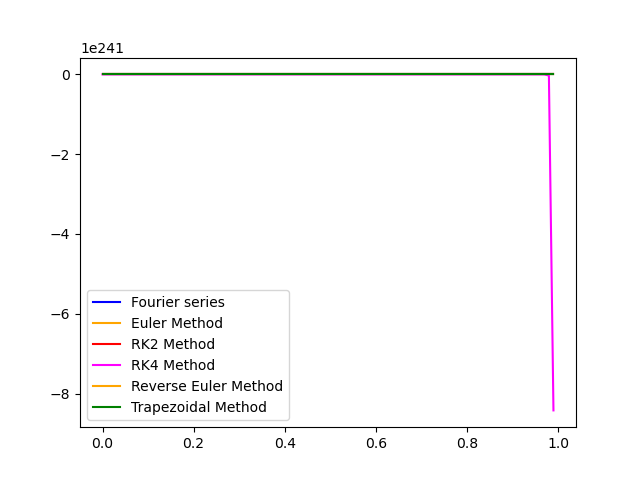
\includegraphics[width=0.45\textwidth]{figs/everything_R1000_L1_h0.01.png}
    }
    \subfloat[All Methods Error]{
        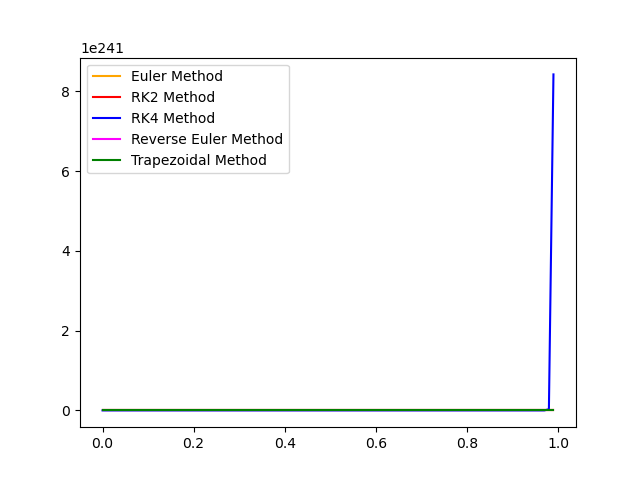
\includegraphics[width=0.45\textwidth]{figs/everythingError_R1000_L1_h0.01.png}
    }
    \caption{Comparison of All Methods (R = 1000 $\Omega$, L = 1 H, h = T/10)}
\end{figure}

\subsection{Time Step h = T/1000}

\begin{figure}[H]
    \centering
    \subfloat[Fourier vs Euler]{
        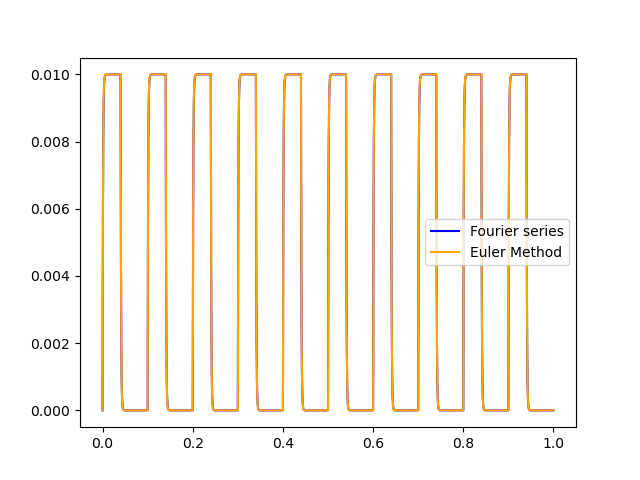
\includegraphics[width=0.45\textwidth]{figs/euler_R1000_L1_h0.0001.png}
    }
    \subfloat[Euler Error]{
        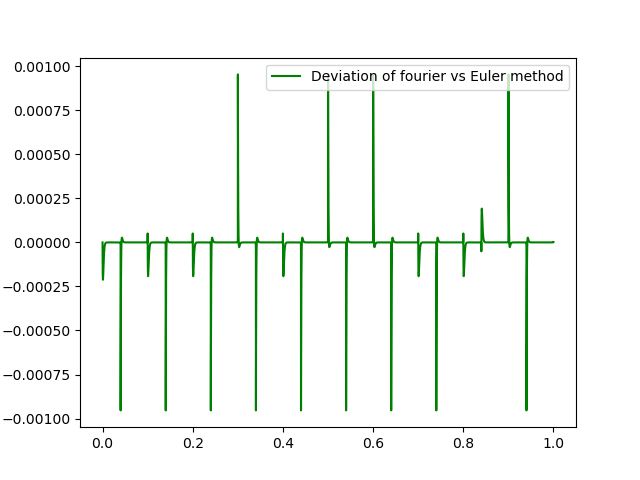
\includegraphics[width=0.45\textwidth]{figs/eulerError_R1000_L1_h0.0001.png}
    }
    \caption{Euler Method Comparison (R = 1000 $\Omega$, L = 1 H, h = T/1000)}
\end{figure}

\begin{figure}[H]
    \centering
    \subfloat[Fourier vs RK2]{
        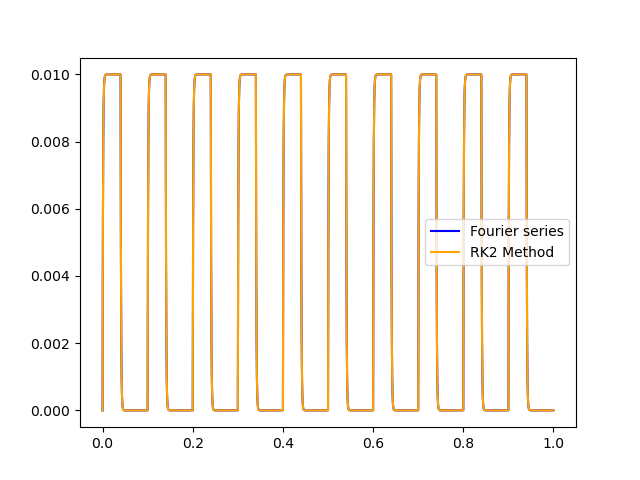
\includegraphics[width=0.45\textwidth]{figs/rk2_R1000_L1_h0.0001.png}
    }
    \subfloat[RK2 Error]{
        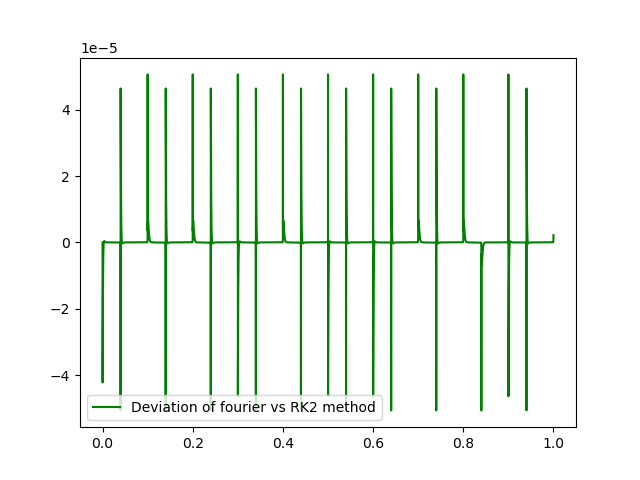
\includegraphics[width=0.45\textwidth]{figs/rk2Error_R1000_L1_h0.0001.png}
    }
    \caption{RK2 Method Comparison (R = 1000 $\Omega$, L = 1 H, h = T/1000)}
\end{figure}

\begin{figure}[H]
    \centering
    \subfloat[Fourier vs RK4]{
        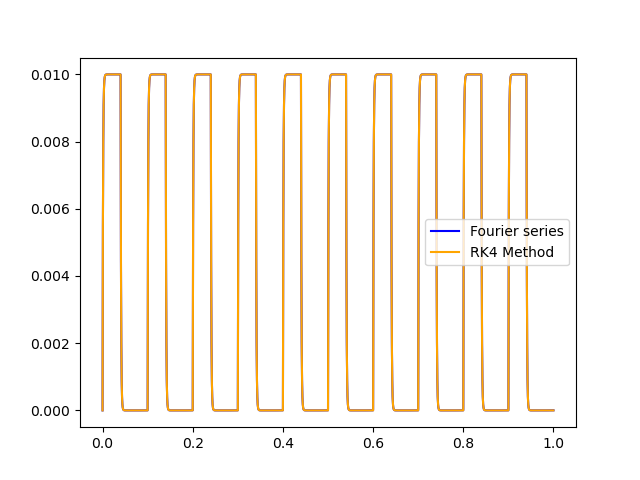
\includegraphics[width=0.45\textwidth]{figs/rk4_R1000_L1_h0.0001.png}
    }
    \subfloat[RK4 Error]{
        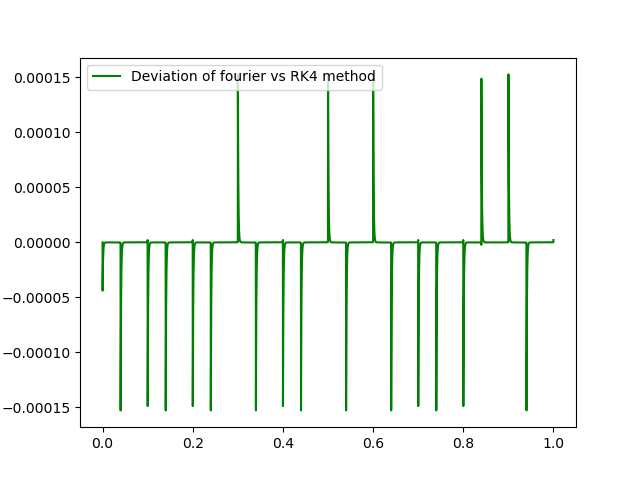
\includegraphics[width=0.45\textwidth]{figs/rk4Error_R1000_L1_h0.0001.png}
    }
    \caption{RK4 Method Comparison (R = 1000 $\Omega$, L = 1 H, h = T/1000)}
\end{figure}

\begin{figure}[H]
    \centering
    \subfloat[Fourier vs Reverse Euler]{
        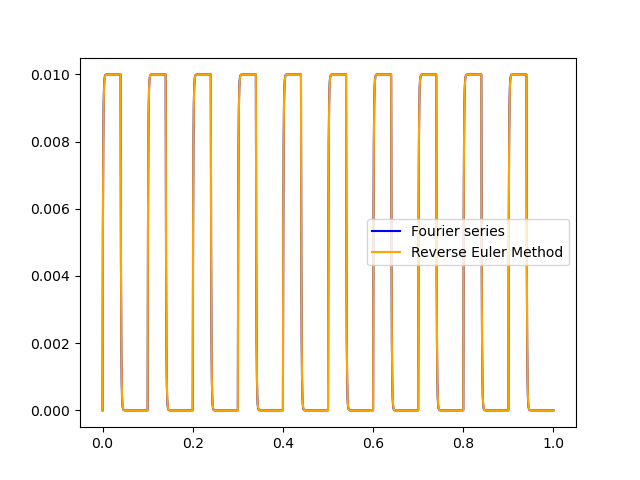
\includegraphics[width=0.45\textwidth]{figs/reverseEuler_R1000_L1_h0.0001.png}
    }
    \subfloat[Reverse Euler Error]{
        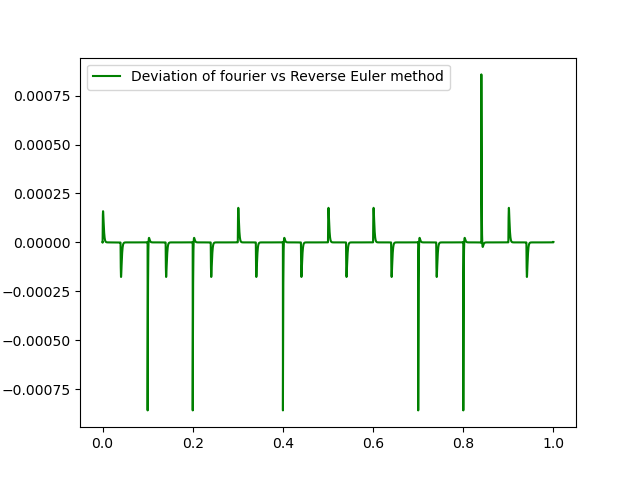
\includegraphics[width=0.45\textwidth]{figs/reverseEulerError_R1000_L1_h0.0001.png}
    }
    \caption{Reverse Euler Method Comparison (R = 1000 $\Omega$, L = 1 H, h = T/1000)}
\end{figure}

\begin{figure}[H]
    \centering
    \subfloat[Fourier vs Trapezoidal]{
        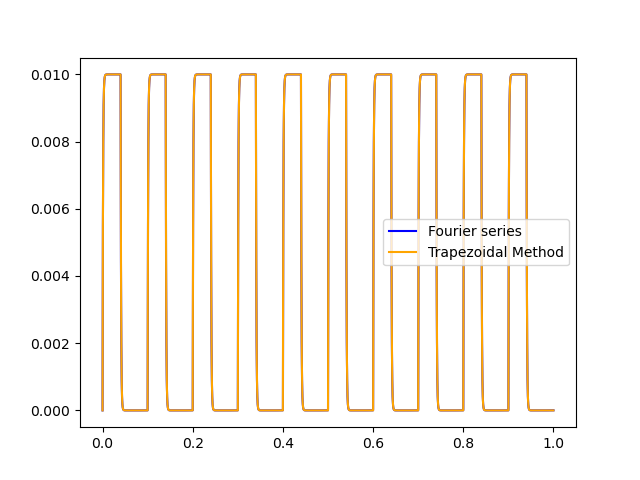
\includegraphics[width=0.45\textwidth]{figs/trapezoidal_R1000_L1_h0.0001.png}
    }
    \subfloat[Trapezoidal Error]{
        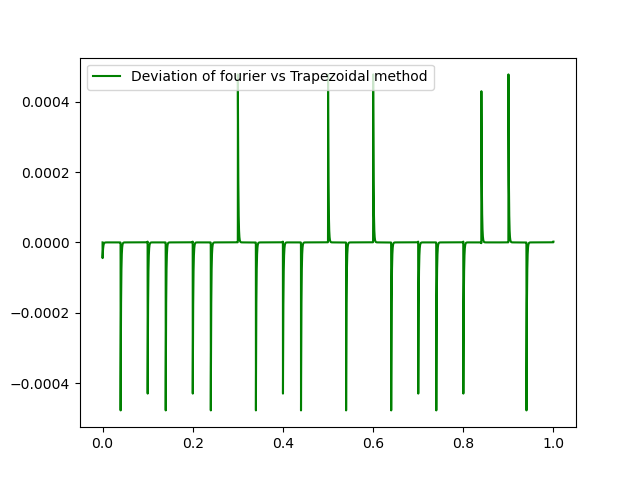
\includegraphics[width=0.45\textwidth]{figs/trapezoidalError_R1000_L1_h0.0001.png}
    }
    \caption{Trapezoidal Method Comparison (R = 1000 $\Omega$, L = 1 H, h = T/1000)}
\end{figure}

\begin{figure}[H]
    \centering
    \subfloat[All Methods Comparison]{
        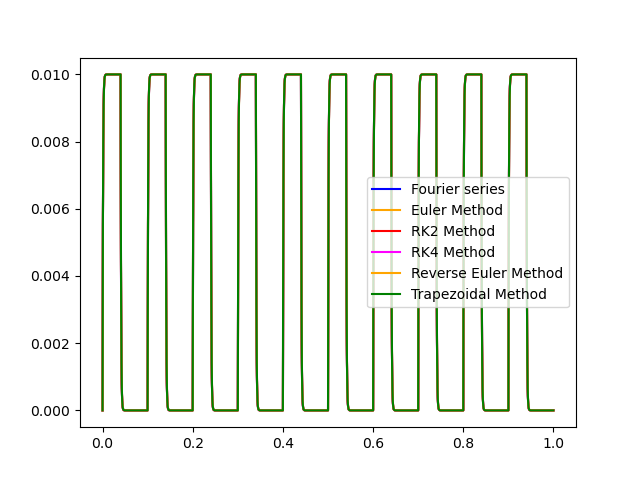
\includegraphics[width=0.45\textwidth]{figs/everything_R1000_L1_h0.0001.png}
    }
    \subfloat[All Methods Error]{
        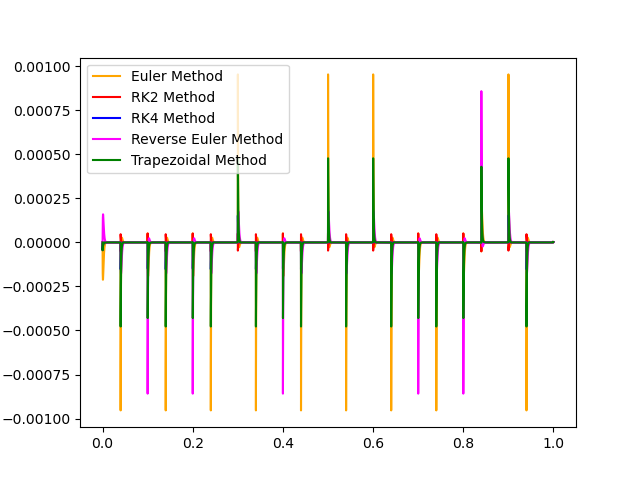
\includegraphics[width=0.45\textwidth]{figs/everythingError_R1000_L1_h0.0001.png}
    }
    \caption{Comparison of All Methods (R = 1000 $\Omega$, L = 1 H, h = T/1000)}
\end{figure}

\section{Results for R = 100 $\Omega$}

\subsection{Time Step h = T/10}

\begin{figure}[H]
    \centering
    \subfloat[Fourier vs Euler]{
        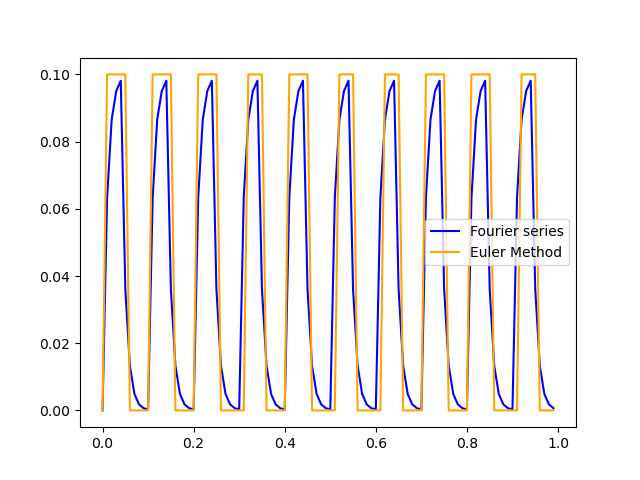
\includegraphics[width=0.45\textwidth]{figs/euler_R100_L1_h0.01.png}
    }
    \subfloat[Euler Error]{
        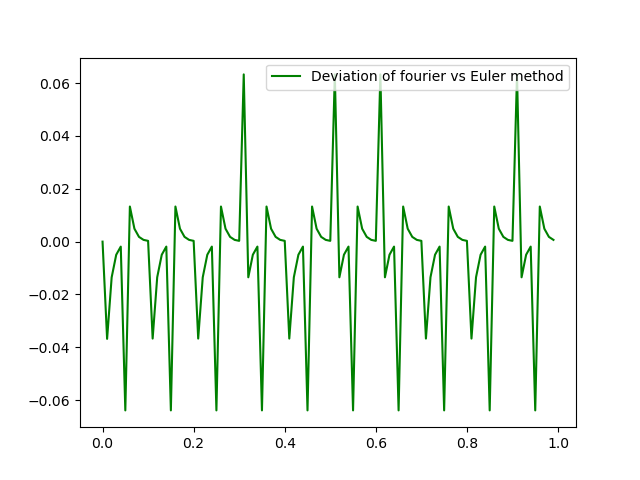
\includegraphics[width=0.45\textwidth]{figs/eulerError_R100_L1_h0.01.png}
    }
    \caption{Euler Method Comparison (R = 100 $\Omega$, L = 1 H, h = T/10)}
\end{figure}

\begin{figure}[H]
    \centering
    \subfloat[Fourier vs RK2]{
        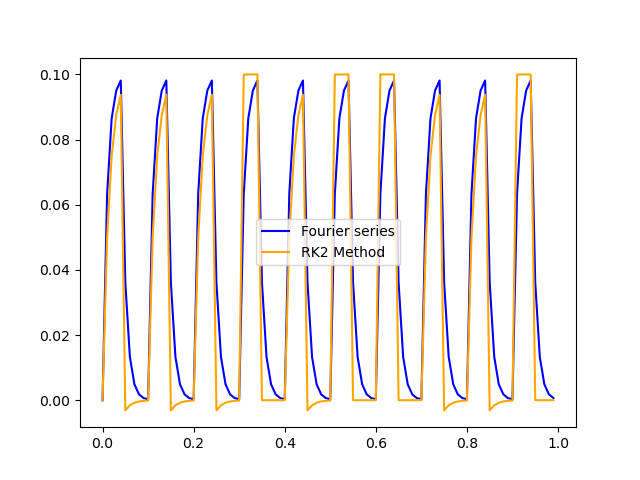
\includegraphics[width=0.45\textwidth]{figs/rk2_R100_L1_h0.01.png}
    }
    \subfloat[RK2 Error]{
        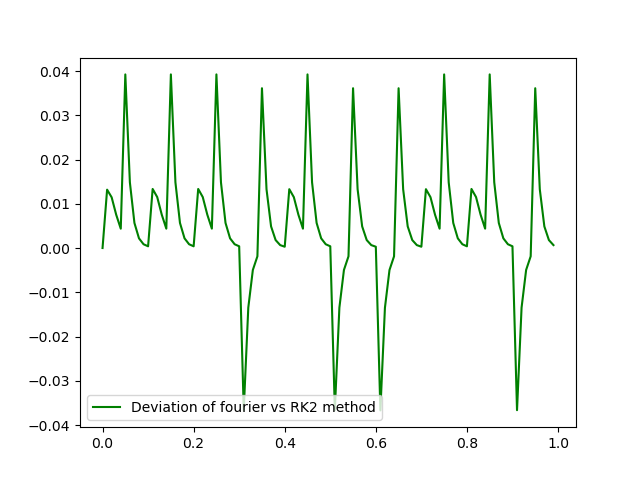
\includegraphics[width=0.45\textwidth]{figs/rk2Error_R100_L1_h0.01.png}
    }
    \caption{RK2 Method Comparison (R = 100 $\Omega$, L = 1 H, h = T/10)}
\end{figure}

\begin{figure}[H]
    \centering
    \subfloat[Fourier vs RK4]{
        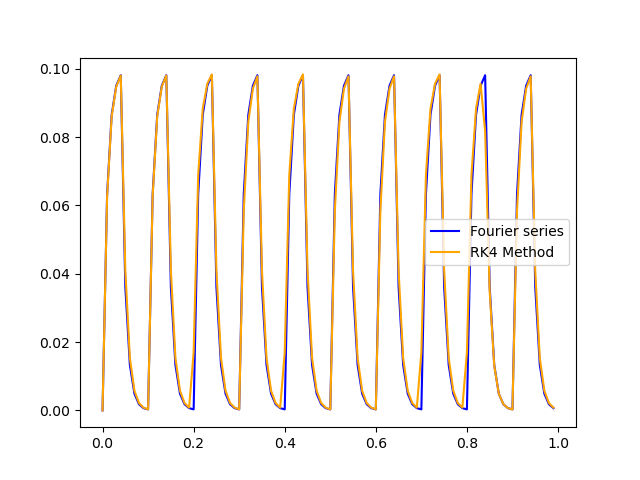
\includegraphics[width=0.45\textwidth]{figs/rk4_R100_L1_h0.01.png}
    }
    \subfloat[RK4 Error]{
        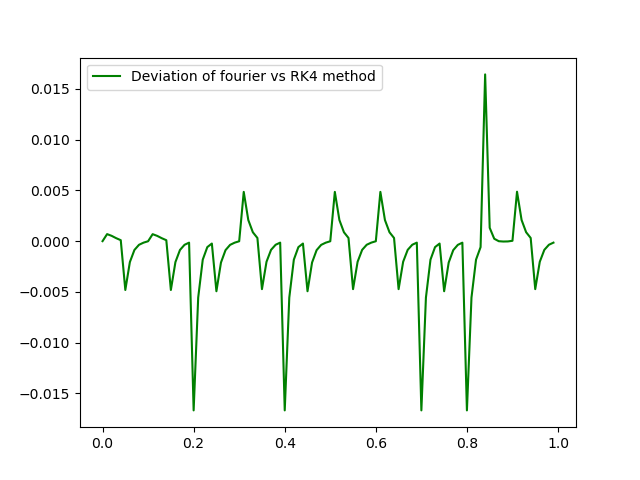
\includegraphics[width=0.45\textwidth]{figs/rk4Error_R100_L1_h0.01.png}
    }
    \caption{RK4 Method Comparison (R = 100 $\Omega$, L = 1 H, h = T/10)}
\end{figure}

\begin{figure}[H]
    \centering
    \subfloat[Fourier vs Reverse Euler]{
        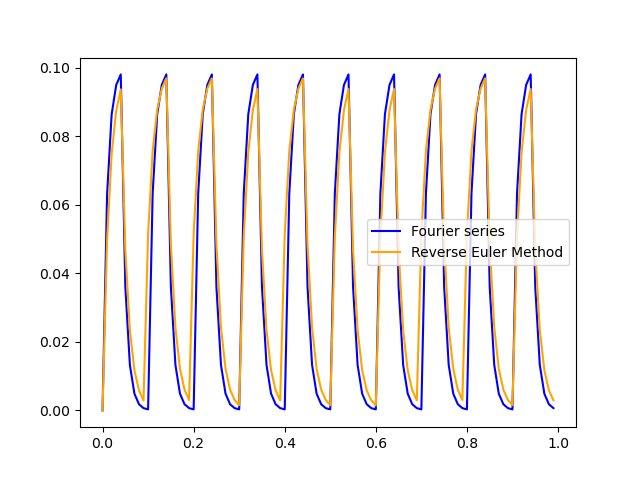
\includegraphics[width=0.45\textwidth]{figs/reverseEuler_R100_L1_h0.01.png}
    }
    \subfloat[Reverse Euler Error]{
        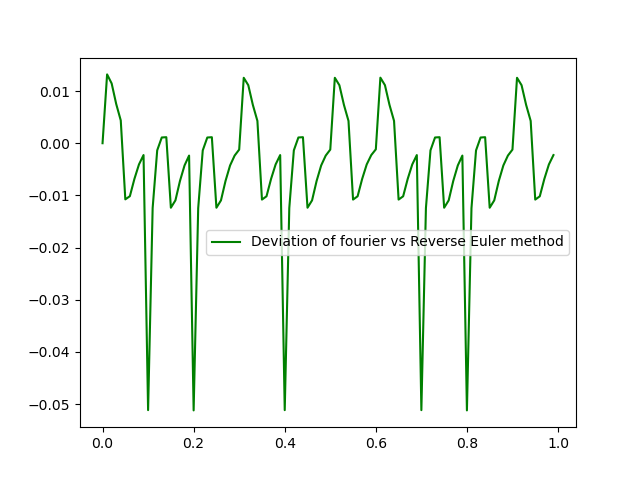
\includegraphics[width=0.45\textwidth]{figs/reverseEulerError_R100_L1_h0.01.png}
    }
    \caption{Reverse Euler Method Comparison (R = 100 $\Omega$, L = 1 H, h = T/10)}
\end{figure}

\begin{figure}[H]
    \centering
    \subfloat[Fourier vs Trapezoidal]{
        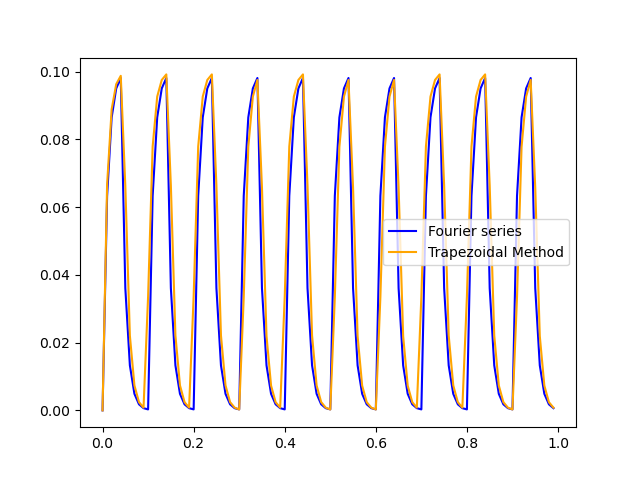
\includegraphics[width=0.45\textwidth]{figs/trapezoidal_R100_L1_h0.01.png}
    }
    \subfloat[Trapezoidal Error]{
        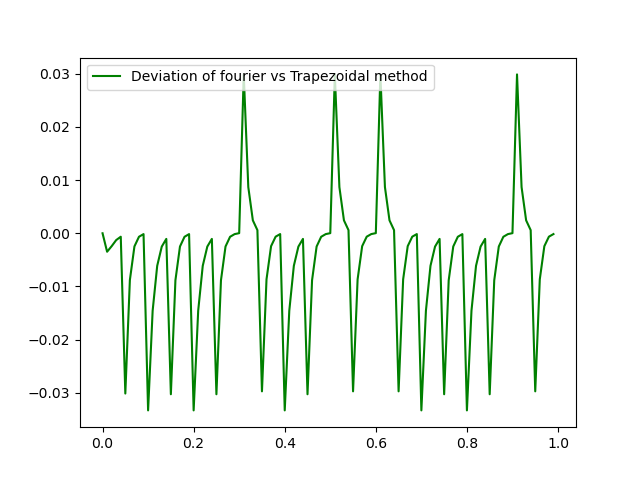
\includegraphics[width=0.45\textwidth]{figs/trapezoidalError_R100_L1_h0.01.png}
    }
    \caption{Trapezoidal Method Comparison (R = 100 $\Omega$, L = 1 H, h = T/10)}
\end{figure}

\begin{figure}[H]
    \centering
    \subfloat[All Methods Comparison]{
        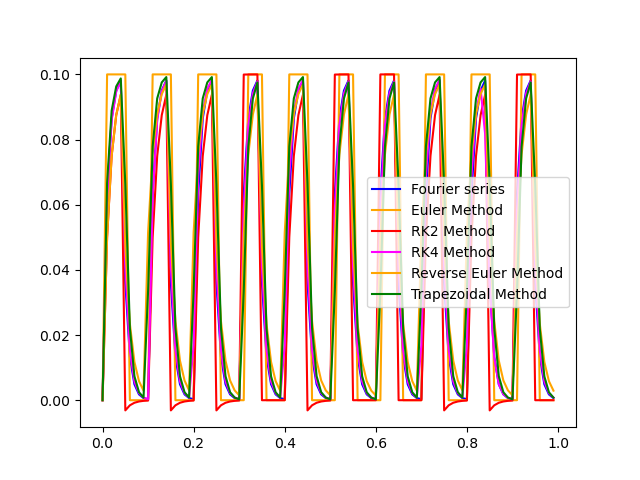
\includegraphics[width=0.45\textwidth]{figs/everything_R100_L1_h0.01.png}
    }
    \subfloat[All Methods Error]{
        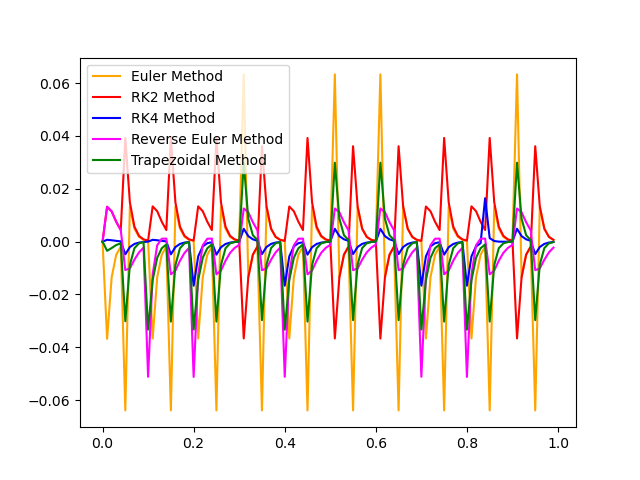
\includegraphics[width=0.45\textwidth]{figs/everythingError_R100_L1_h0.01.png}
    }
    \caption{Comparison of All Methods (R = 100 $\Omega$, L = 1 H, h = T/10)}
\end{figure}

\subsection{Time Step h = T/1000}

\begin{figure}[H]
    \centering
    \subfloat[Fourier vs Euler]{
        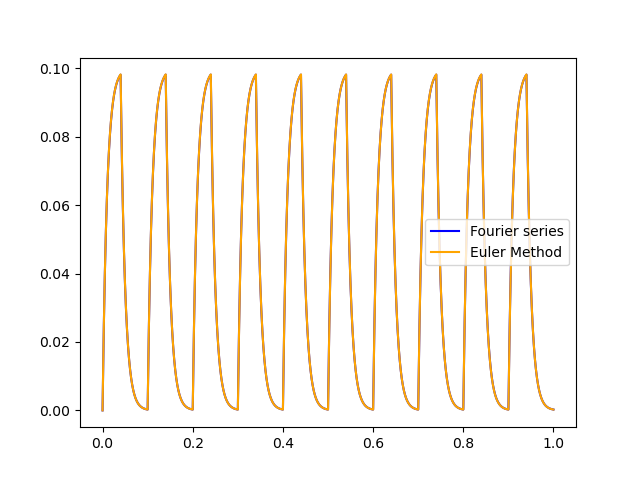
\includegraphics[width=0.45\textwidth]{figs/euler_R100_L1_h0.0001.png}
    }
    \subfloat[Euler Error]{
        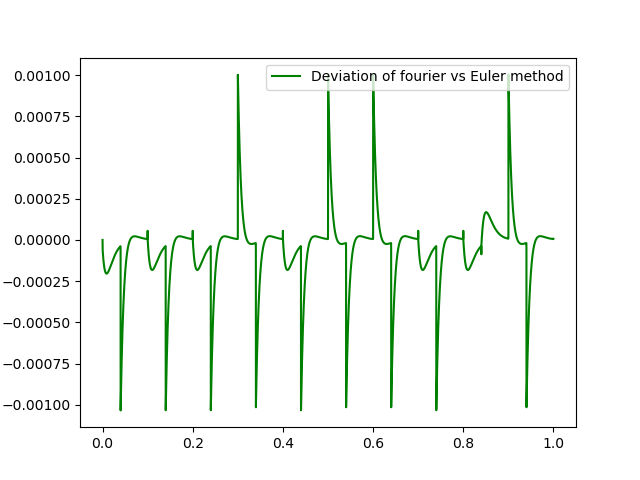
\includegraphics[width=0.45\textwidth]{figs/eulerError_R100_L1_h0.0001.png}
    }
    \caption{Euler Method Comparison (R = 100 $\Omega$, L = 1 H, h = T/1000)}
\end{figure}

\begin{figure}[H]
    \centering
    \subfloat[Fourier vs RK2]{
        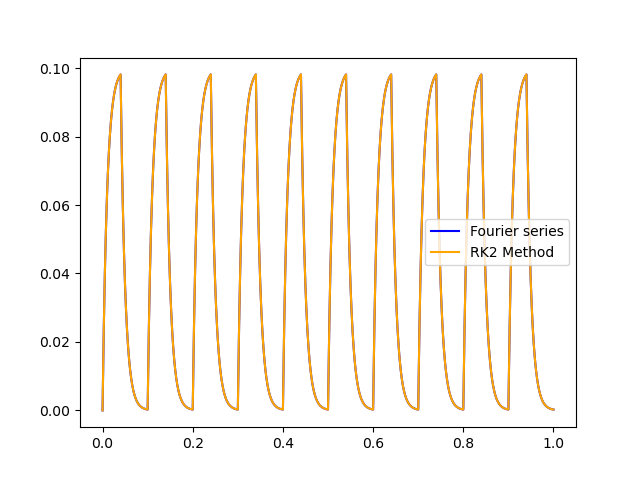
\includegraphics[width=0.45\textwidth]{figs/rk2_R100_L1_h0.0001.png}
    }
    \subfloat[RK2 Error]{
        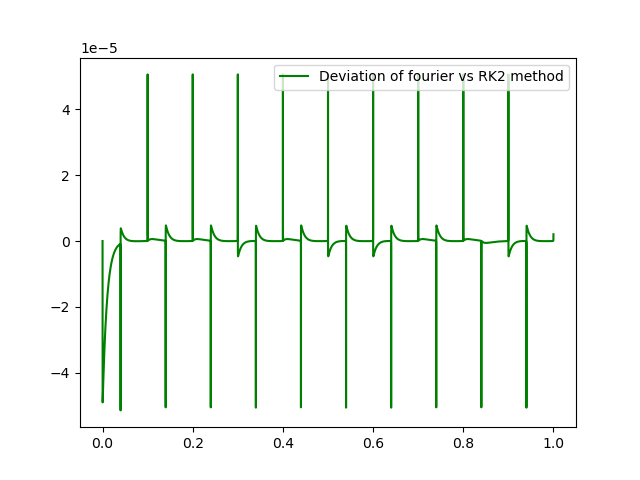
\includegraphics[width=0.45\textwidth]{figs/rk2Error_R100_L1_h0.0001.png}
    }
    \caption{RK2 Method Comparison (R = 100 $\Omega$, L = 1 H, h = T/1000)}
\end{figure}

\begin{figure}[H]
    \centering
    \subfloat[Fourier vs RK4]{
        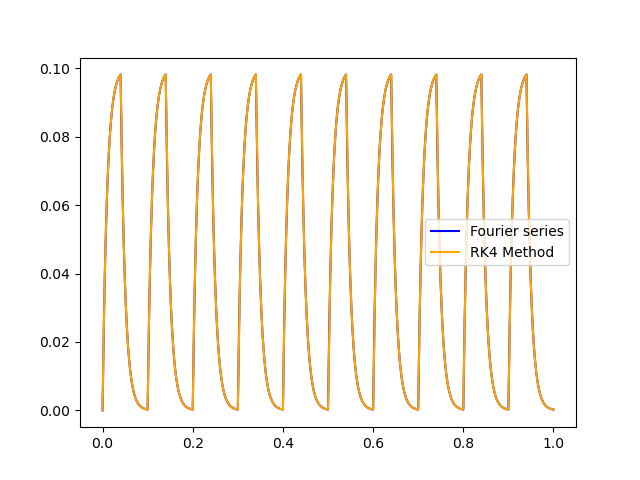
\includegraphics[width=0.45\textwidth]{figs/rk4_R100_L1_h0.0001.png}
    }
    \subfloat[RK4 Error]{
        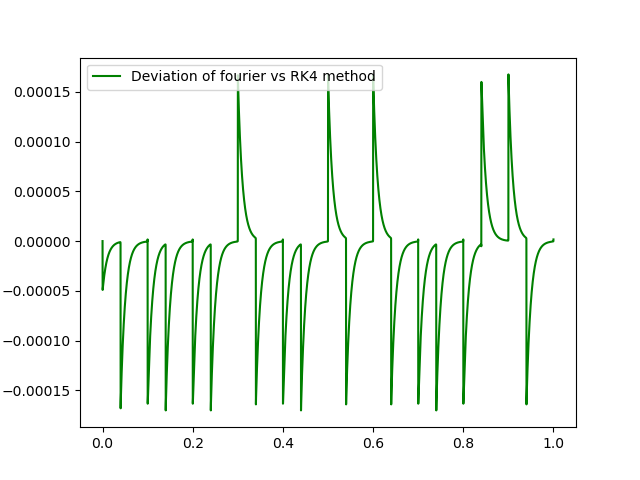
\includegraphics[width=0.45\textwidth]{figs/rk4Error_R100_L1_h0.0001.png}
    }
    \caption{RK4 Method Comparison (R = 100 $\Omega$, L = 1 H, h = T/1000)}
\end{figure}

\begin{figure}[H]
    \centering
    \subfloat[Fourier vs Reverse Euler]{
        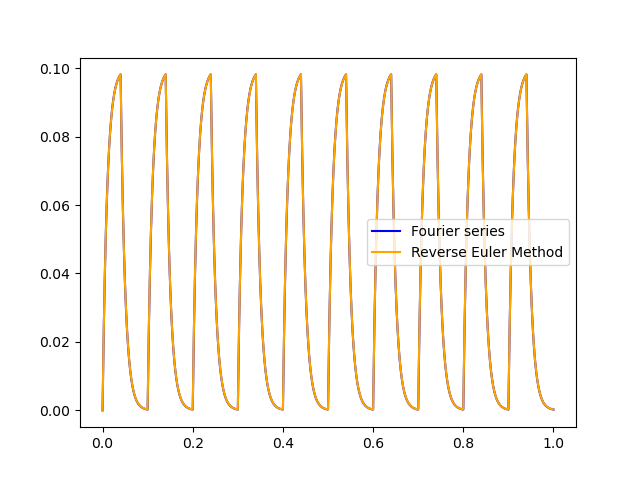
\includegraphics[width=0.45\textwidth]{figs/reverseEuler_R100_L1_h0.0001.png}
    }
    \subfloat[Reverse Euler Error]{
        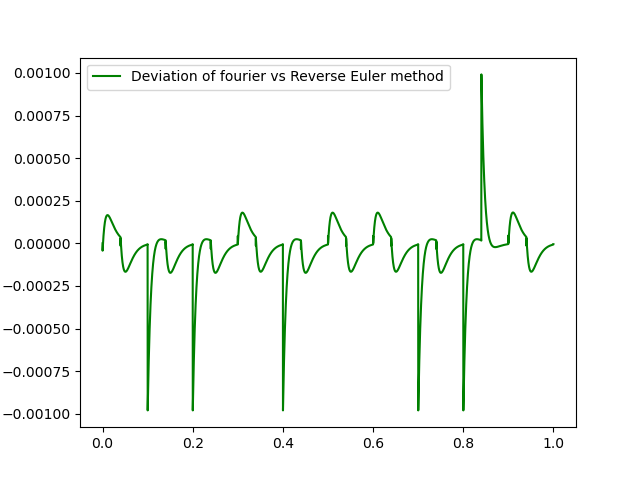
\includegraphics[width=0.45\textwidth]{figs/reverseEulerError_R100_L1_h0.0001.png}
    }
    \caption{Reverse Euler Method Comparison (R = 100 $\Omega$, L = 1 H, h = T/1000)}
\end{figure}

\begin{figure}[H]
    \centering
    \subfloat[Fourier vs Trapezoidal]{
        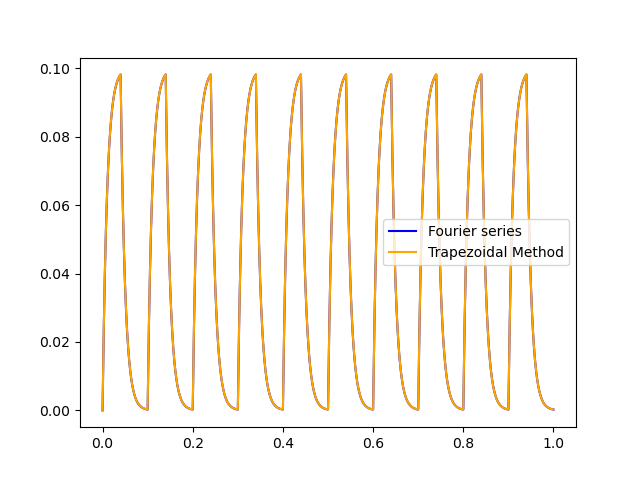
\includegraphics[width=0.45\textwidth]{figs/trapezoidal_R100_L1_h0.0001.png}
    }
    \subfloat[Trapezoidal Error]{
        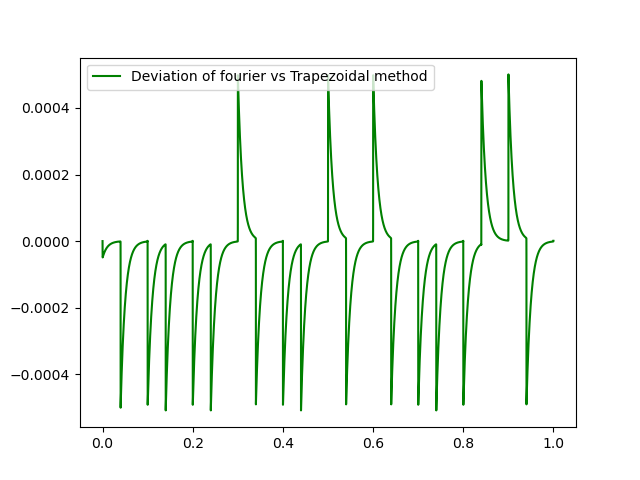
\includegraphics[width=0.45\textwidth]{figs/trapezoidalError_R100_L1_h0.0001.png}
    }
    \caption{Trapezoidal Method Comparison (R = 100 $\Omega$, L = 1 H, h = T/1000)}
\end{figure}

\begin{figure}[H]
    \centering
    \subfloat[All Methods Comparison]{
        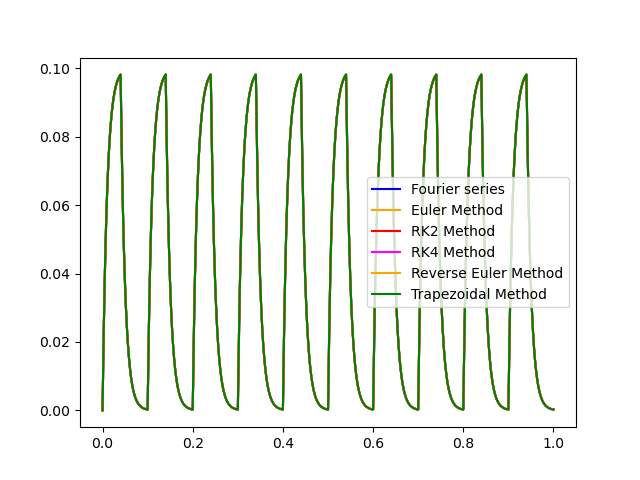
\includegraphics[width=0.45\textwidth]{figs/everything_R100_L1_h0.0001.png}
    }
    \subfloat[All Methods Error]{
        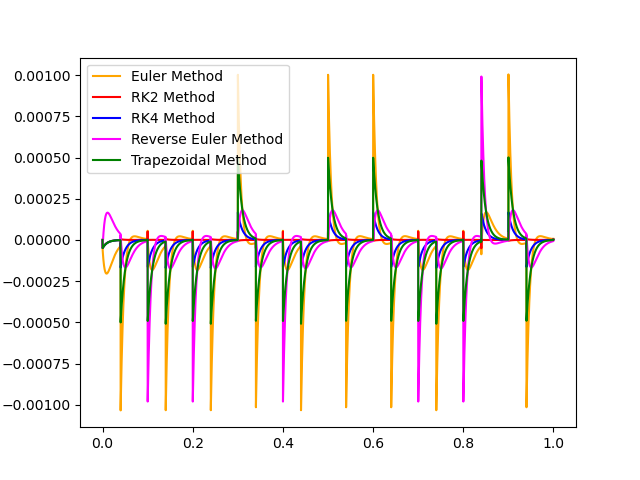
\includegraphics[width=0.45\textwidth]{figs/everythingError_R100_L1_h0.0001.png}
    }
    \caption{Comparison of All Methods (R = 100 $\Omega$, L = 1 H, h = T/1000)}
\end{figure}

\section{Results for R = 1 $\Omega$}

\subsection{Time Step h = T/10}

\begin{figure}[H]
    \centering
    \subfloat[Fourier vs Euler]{
        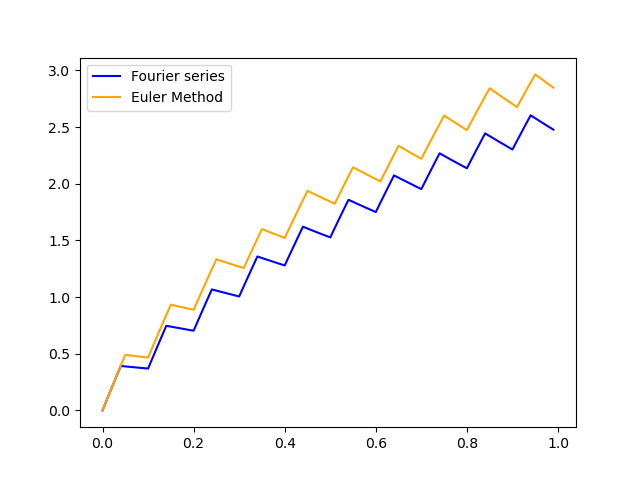
\includegraphics[width=0.45\textwidth]{figs/euler_R1_L1_h0.01.png}
    }
    \subfloat[Euler Error]{
        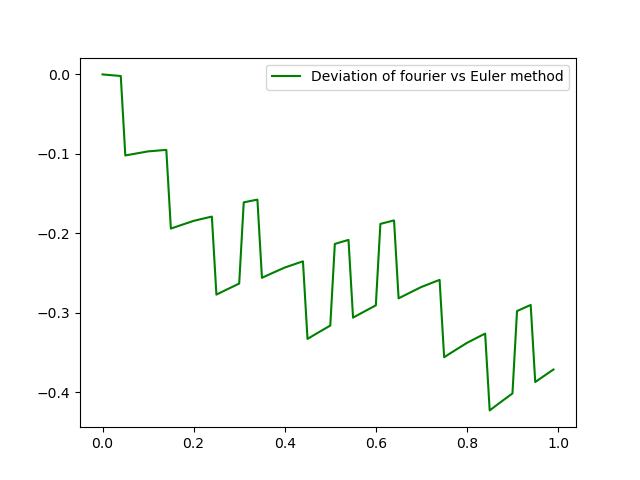
\includegraphics[width=0.45\textwidth]{figs/eulerError_R1_L1_h0.01.png}
    }
    \caption{Euler Method Comparison (R = 1 $\Omega$, L = 1 H, h = T/10)}
\end{figure}

\begin{figure}[H]
    \centering
    \subfloat[Fourier vs RK2]{
        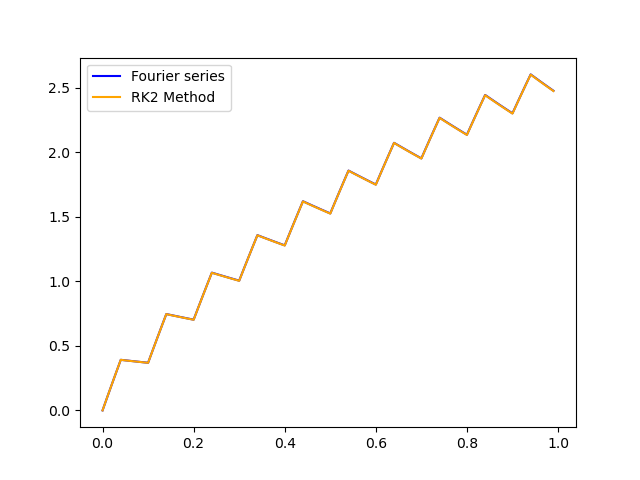
\includegraphics[width=0.45\textwidth]{figs/rk2_R1_L1_h0.01.png}
    }
    \subfloat[RK2 Error]{
        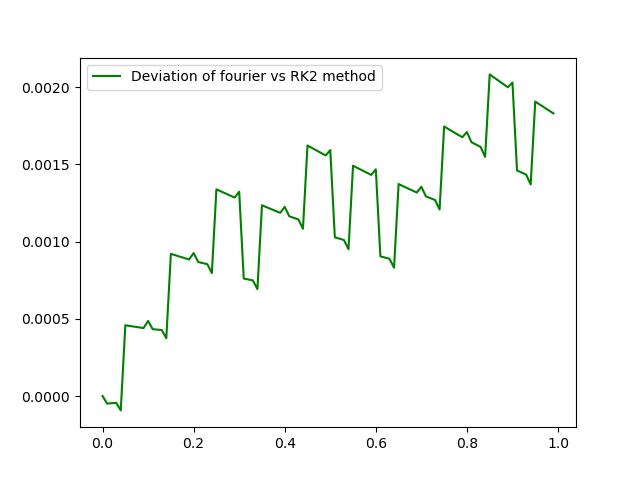
\includegraphics[width=0.45\textwidth]{figs/rk2Error_R1_L1_h0.01.png}
    }
    \caption{RK2 Method Comparison (R = 1 $\Omega$, L = 1 H, h = T/10)}
\end{figure}

\begin{figure}[H]
    \centering
    \subfloat[Fourier vs RK4]{
        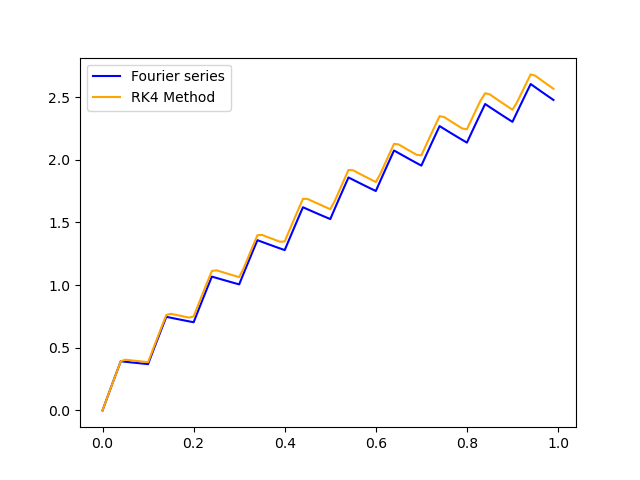
\includegraphics[width=0.45\textwidth]{figs/rk4_R1_L1_h0.01.png}
    }
    \subfloat[RK4 Error]{
        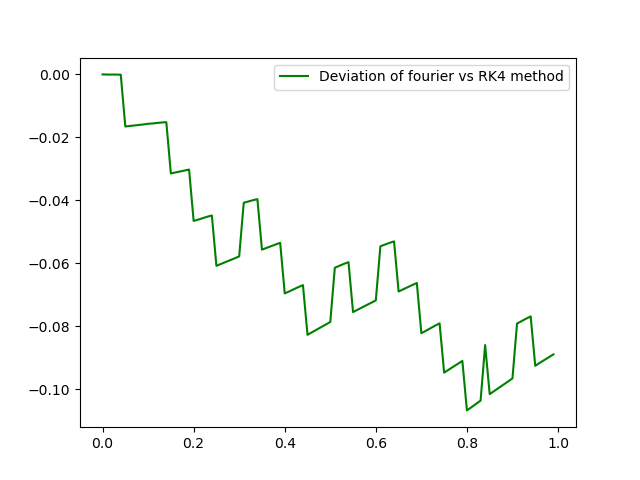
\includegraphics[width=0.45\textwidth]{figs/rk4Error_R1_L1_h0.01.png}
    }
    \caption{RK4 Method Comparison (R = 1 $\Omega$, L = 1 H, h = T/10)}
\end{figure}

\begin{figure}[H]
    \centering
    \subfloat[Fourier vs Reverse Euler]{
        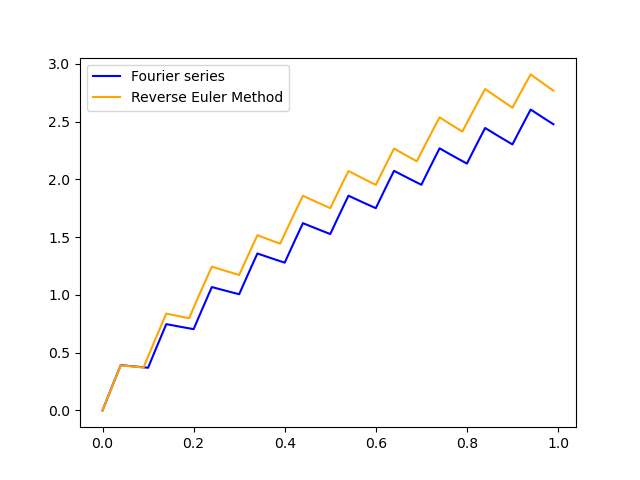
\includegraphics[width=0.45\textwidth]{figs/reverseEuler_R1_L1_h0.01.png}
    }
    \subfloat[Reverse Euler Error]{
        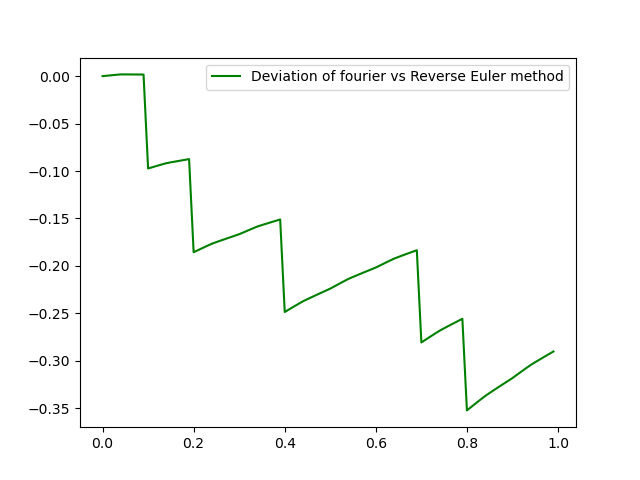
\includegraphics[width=0.45\textwidth]{figs/reverseEulerError_R1_L1_h0.01.png}
    }
    \caption{Reverse Euler Method Comparison (R = 1 $\Omega$, L = 1 H, h = T/10)}
\end{figure}

\begin{figure}[H]
    \centering
    \subfloat[Fourier vs Trapezoidal]{
        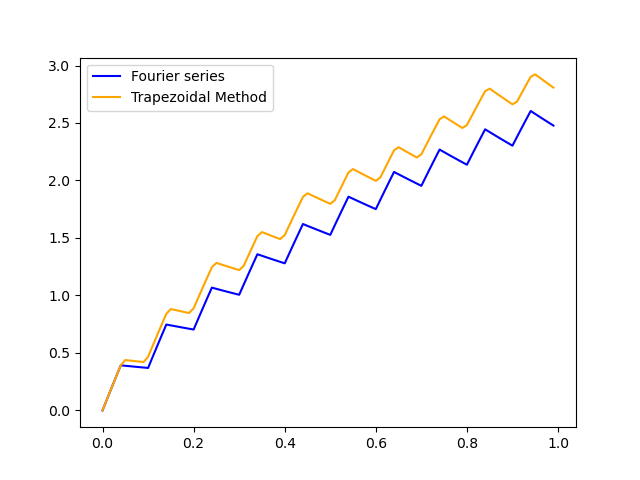
\includegraphics[width=0.45\textwidth]{figs/trapezoidal_R1_L1_h0.01.png}
    }
    \subfloat[Trapezoidal Error]{
        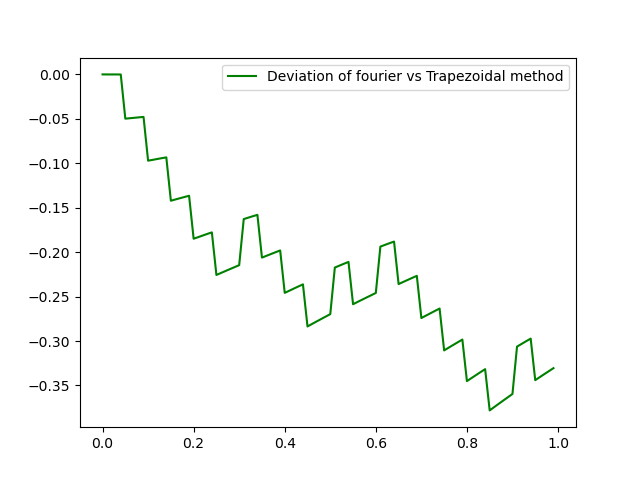
\includegraphics[width=0.45\textwidth]{figs/trapezoidalError_R1_L1_h0.01.png}
    }
    \caption{Trapezoidal Method Comparison (R = 1 $\Omega$, L = 1 H, h = T/10)}
\end{figure}

\begin{figure}[H]
    \centering
    \subfloat[All Methods Comparison]{
        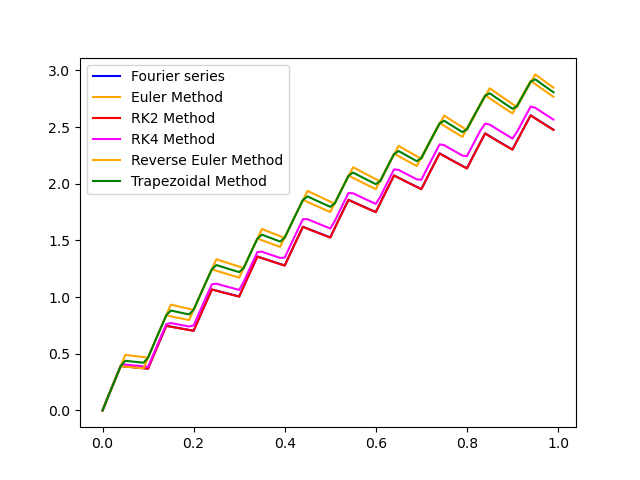
\includegraphics[width=0.45\textwidth]{figs/everything_R1_L1_h0.01.png}
    }
    \subfloat[All Methods Error]{
        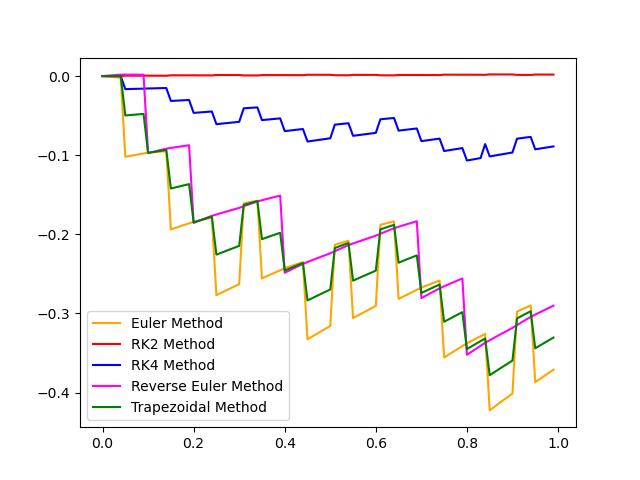
\includegraphics[width=0.45\textwidth]{figs/everythingError_R1_L1_h0.01.png}
    }
    \caption{Comparison of All Methods (R = 1 $\Omega$, L = 1 H, h = T/10)}
\end{figure}

\subsection{Time Step h = T/1000}

\begin{figure}[H]
    \centering
    \subfloat[Fourier vs Euler]{
        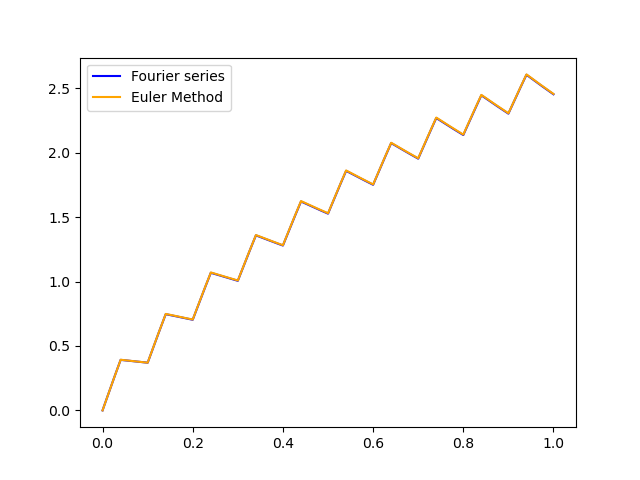
\includegraphics[width=0.45\textwidth]{figs/euler_R1_L1_h0.0001.png}
    }
    \subfloat[Euler Error]{
        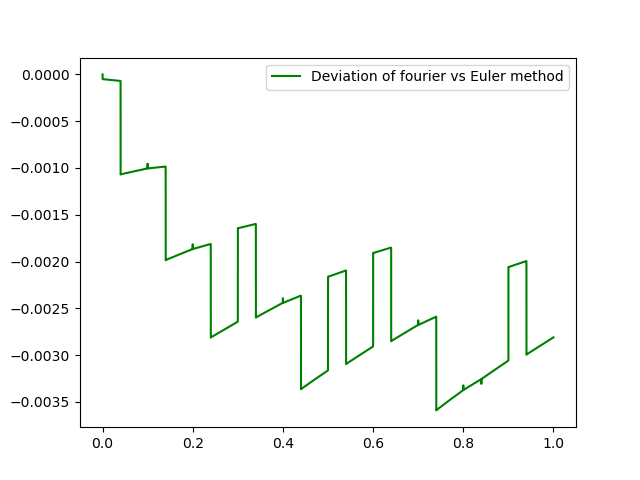
\includegraphics[width=0.45\textwidth]{figs/eulerError_R1_L1_h0.0001.png}
    }
    \caption{Euler Method Comparison (R = 1 $\Omega$, L = 1 H, h = T/1000)}
\end{figure}

\begin{figure}[H]
    \centering
    \subfloat[Fourier vs RK2]{
        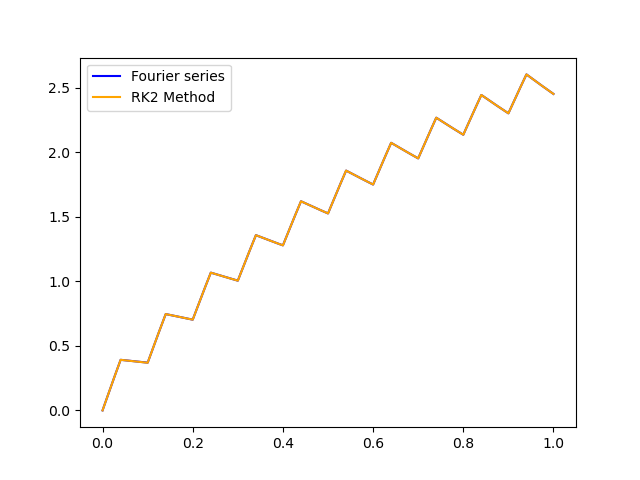
\includegraphics[width=0.45\textwidth]{figs/rk2_R1_L1_h0.0001.png}
    }
    \subfloat[RK2 Error]{
        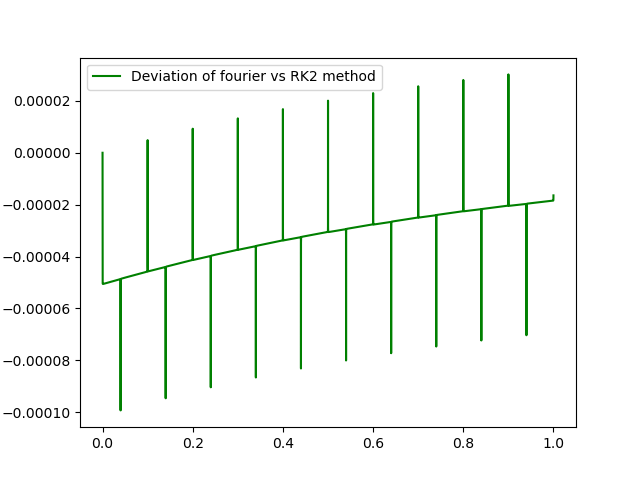
\includegraphics[width=0.45\textwidth]{figs/rk2Error_R1_L1_h0.0001.png}
    }
    \caption{RK2 Method Comparison (R = 1 $\Omega$, L = 1 H, h = T/1000)}
\end{figure}

\begin{figure}[H]
    \centering
    \subfloat[Fourier vs RK4]{
        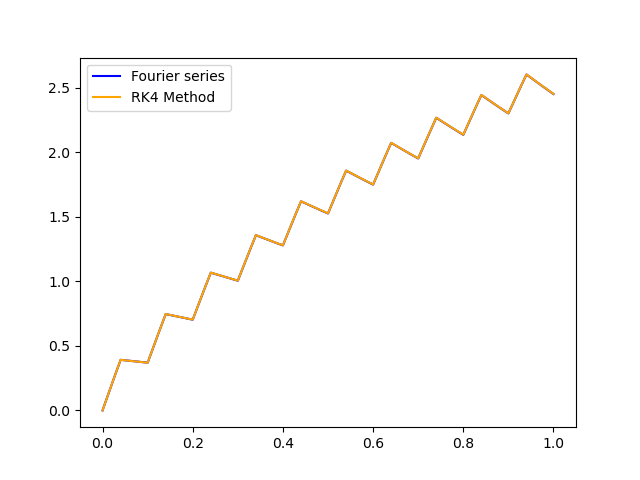
\includegraphics[width=0.45\textwidth]{figs/rk4_R1_L1_h0.0001.png}
    }
    \subfloat[RK4 Error]{
        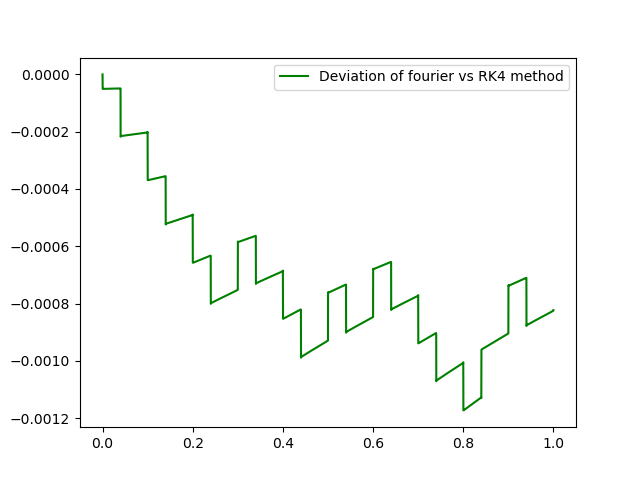
\includegraphics[width=0.45\textwidth]{figs/rk4Error_R1_L1_h0.0001.png}
    }
    \caption{RK4 Method Comparison (R = 1 $\Omega$, L = 1 H, h = T/1000)}
\end{figure}

\begin{figure}[H]
    \centering
    \subfloat[Fourier vs Reverse Euler]{
        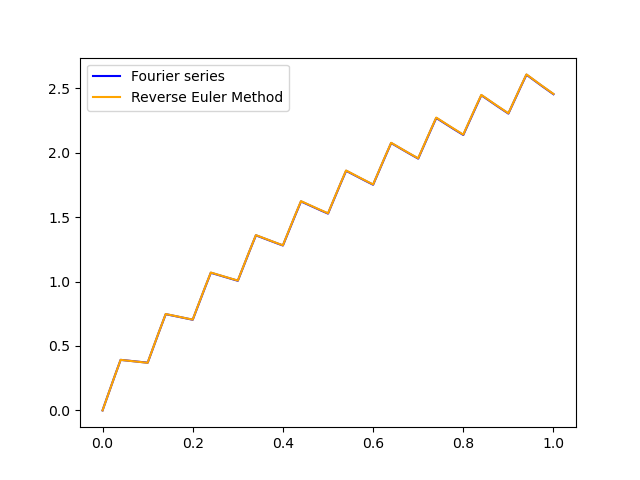
\includegraphics[width=0.45\textwidth]{figs/reverseEuler_R1_L1_h0.0001.png}
    }
    \subfloat[Reverse Euler Error]{
        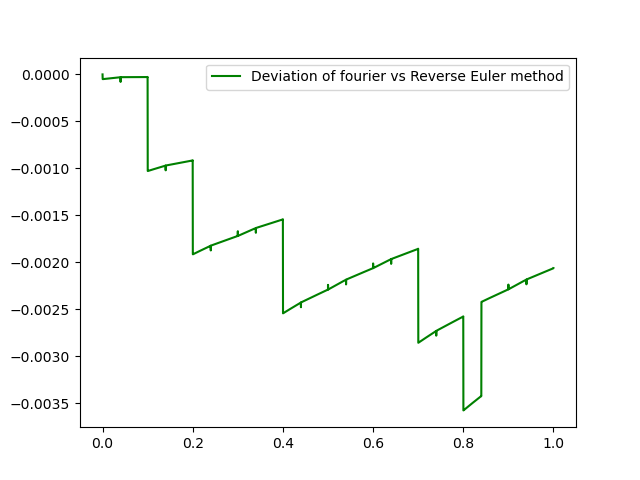
\includegraphics[width=0.45\textwidth]{figs/reverseEulerError_R1_L1_h0.0001.png}
    }
    \caption{Reverse Euler Method Comparison (R = 1 $\Omega$, L = 1 H, h = T/1000)}
\end{figure}

\begin{figure}[H]
    \centering
    \subfloat[Fourier vs Trapezoidal]{
        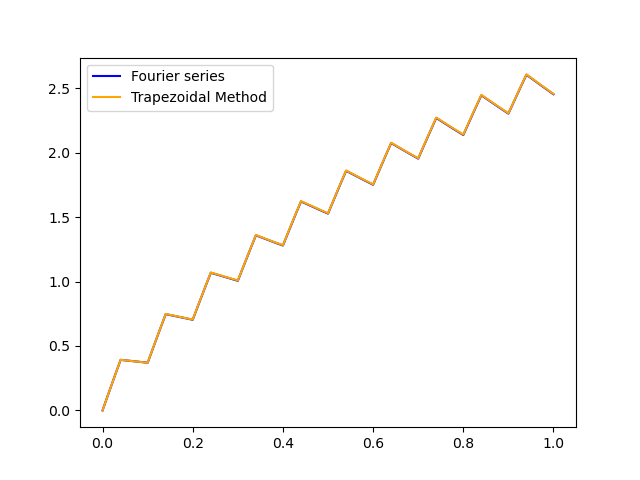
\includegraphics[width=0.45\textwidth]{figs/trapezoidal_R1_L1_h0.0001.png}
    }
    \subfloat[Trapezoidal Error]{
        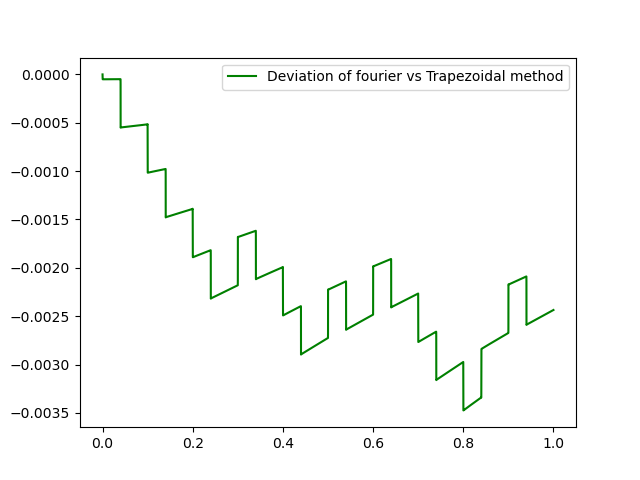
\includegraphics[width=0.45\textwidth]{figs/trapezoidalError_R1_L1_h0.0001.png}
    }
    \caption{Trapezoidal Method Comparison (R = 1 $\Omega$, L = 1 H, h = T/1000)}
\end{figure}

\begin{figure}[H]
    \centering
    \subfloat[All Methods Comparison]{
        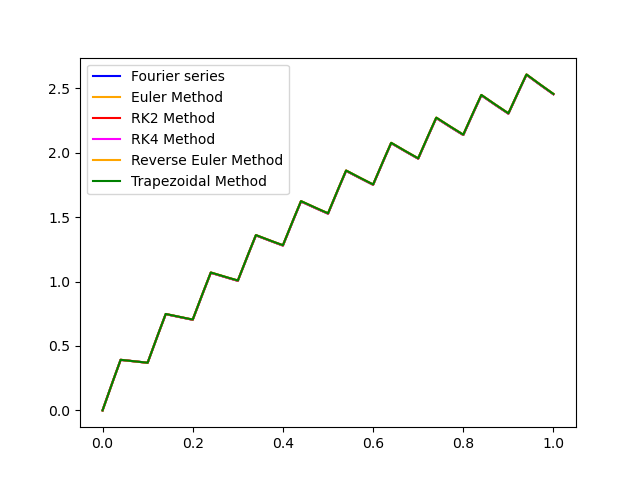
\includegraphics[width=0.45\textwidth]{figs/everything_R1_L1_h0.0001.png}
    }
    \subfloat[All Methods Error]{
        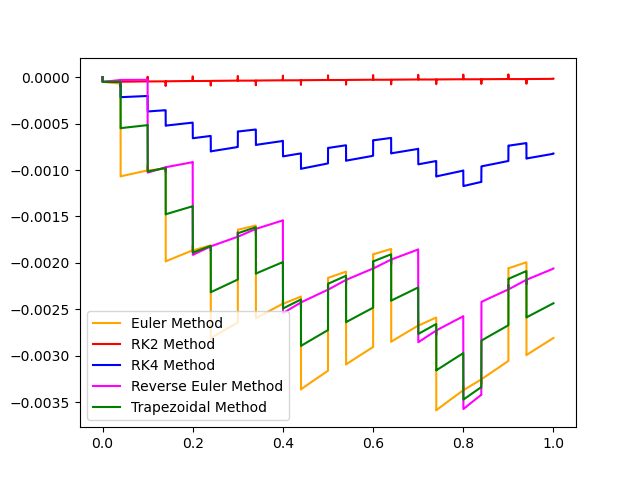
\includegraphics[width=0.45\textwidth]{figs/everythingError_R1_L1_h0.0001.png}
    }
    \caption{Comparison of All Methods (R = 1 $\Omega$, L = 1 H, h = T/1000)}
\end{figure}

\section{Results for R = 0.001 $\Omega$}

\subsection{Time Step h = T/10}

\begin{figure}[H]
    \centering
    \subfloat[Fourier vs Euler]{
        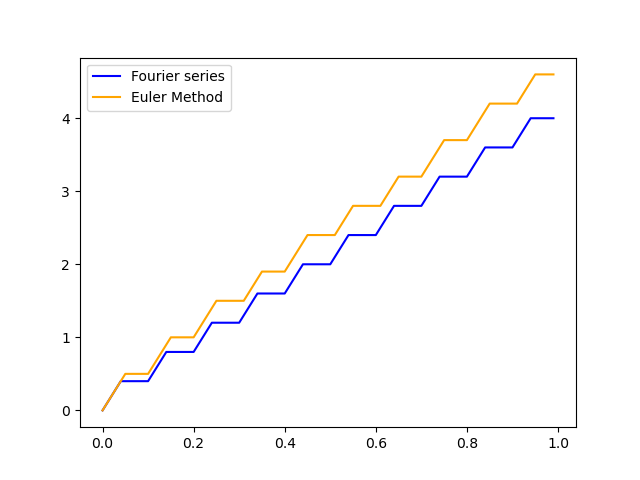
\includegraphics[width=0.45\textwidth]{figs/euler_R0.001_L1_h0.01.png}
    }
    \subfloat[Euler Error]{
        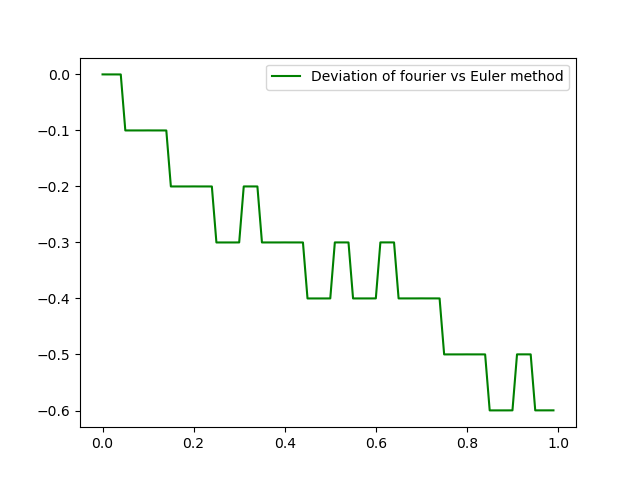
\includegraphics[width=0.45\textwidth]{figs/eulerError_R0.001_L1_h0.01.png}
    }
    \caption{Euler Method Comparison (R = 0.001 $\Omega$, L = 1 H, h = T/10)}
\end{figure}

\begin{figure}[H]
    \centering
    \subfloat[Fourier vs RK2]{
        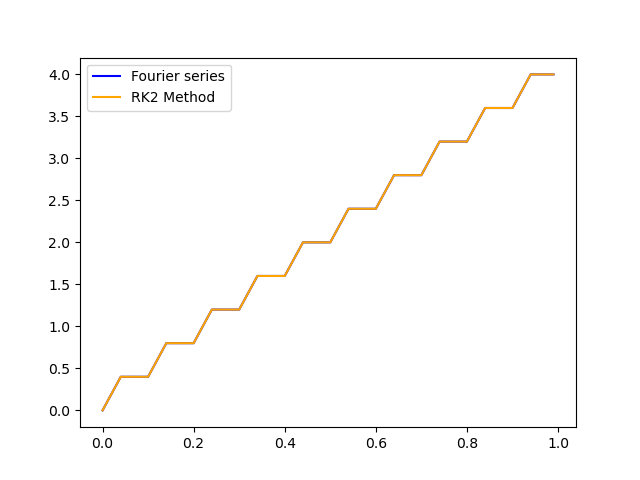
\includegraphics[width=0.45\textwidth]{figs/rk2_R0.001_L1_h0.01.png}
    }
    \subfloat[RK2 Error]{
        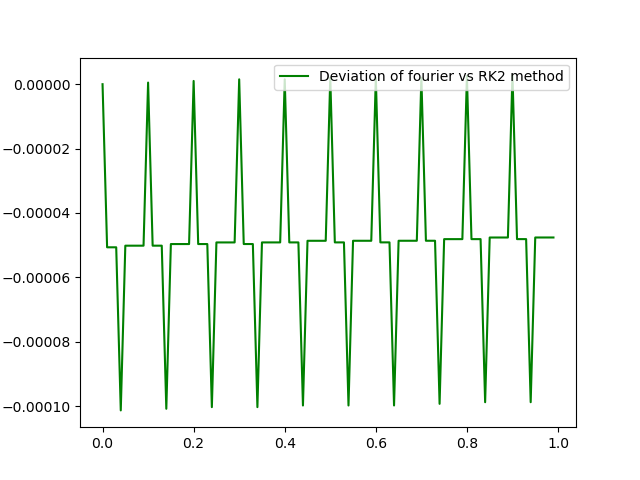
\includegraphics[width=0.45\textwidth]{figs/rk2Error_R0.001_L1_h0.01.png}
    }
    \caption{RK2 Method Comparison (R = 0.001 $\Omega$, L = 1 H, h = T/10)}
\end{figure}

\begin{figure}[H]
    \centering
    \subfloat[Fourier vs RK4]{
        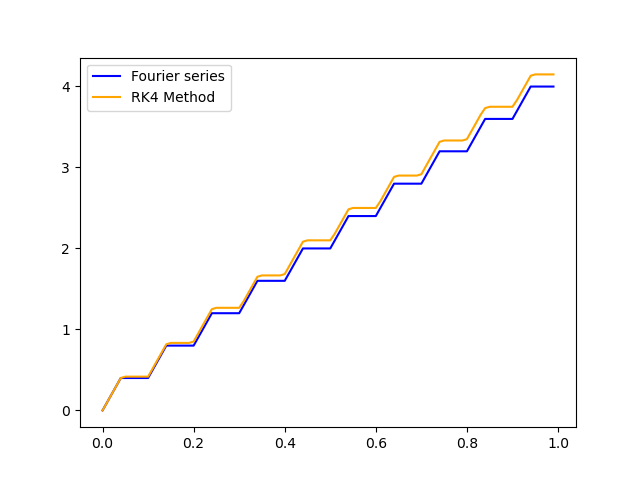
\includegraphics[width=0.45\textwidth]{figs/rk4_R0.001_L1_h0.01.png}
    }
    \subfloat[RK4 Error]{
        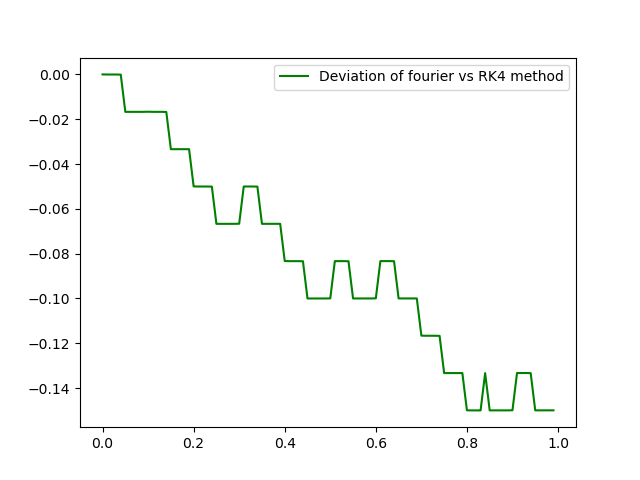
\includegraphics[width=0.45\textwidth]{figs/rk4Error_R0.001_L1_h0.01.png}
    }
    \caption{RK4 Method Comparison (R = 0.001 $\Omega$, L = 1 H, h = T/10)}
\end{figure}

\begin{figure}[H]
    \centering
    \subfloat[Fourier vs Reverse Euler]{
        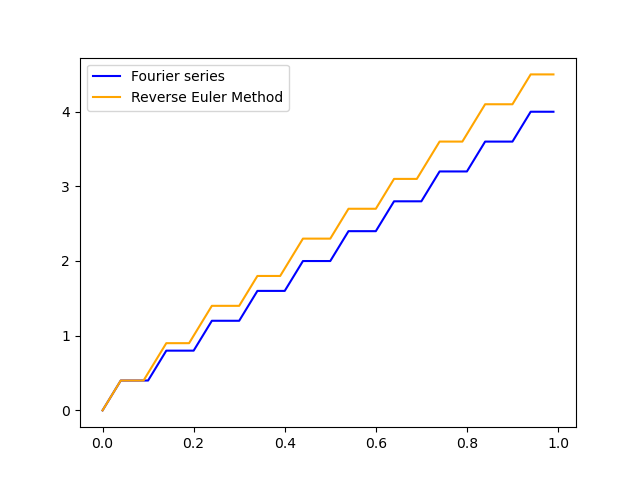
\includegraphics[width=0.45\textwidth]{figs/reverseEuler_R0.001_L1_h0.01.png}
    }
    \subfloat[Reverse Euler Error]{
        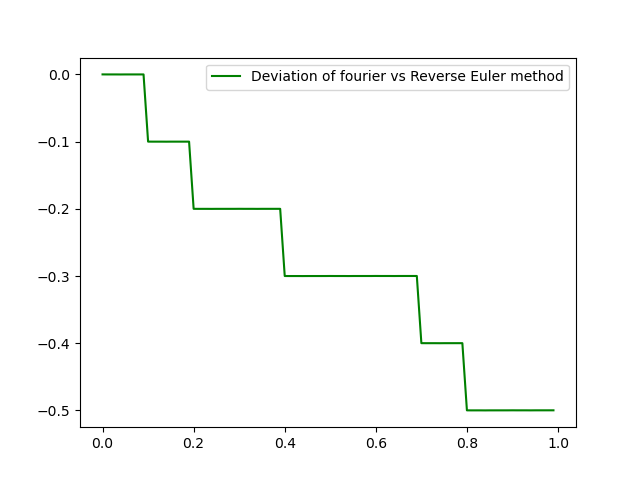
\includegraphics[width=0.45\textwidth]{figs/reverseEulerError_R0.001_L1_h0.01.png}
    }
    \caption{Reverse Euler Method Comparison (R = 0.001 $\Omega$, L = 1 H, h = T/10)}
\end{figure}

\begin{figure}[H]
    \centering
    \subfloat[Fourier vs Trapezoidal]{
        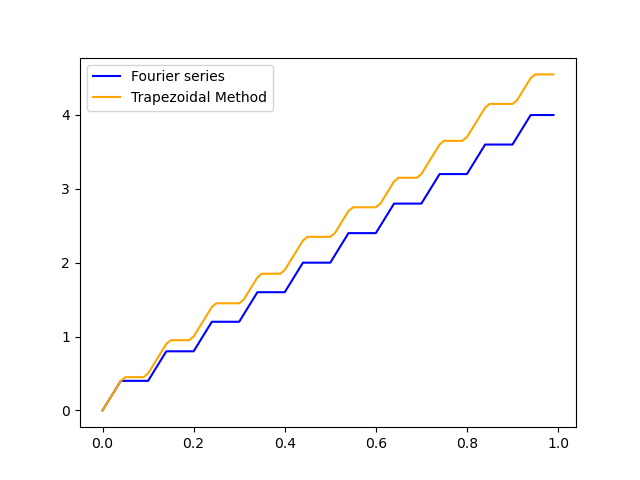
\includegraphics[width=0.45\textwidth]{figs/trapezoidal_R0.001_L1_h0.01.png}
    }
    \subfloat[Trapezoidal Error]{
        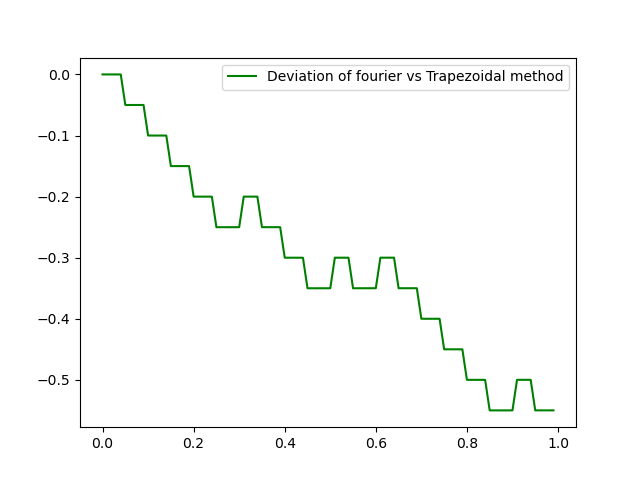
\includegraphics[width=0.45\textwidth]{figs/trapezoidalError_R0.001_L1_h0.01.png}
    }
    \caption{Trapezoidal Method Comparison (R = 0.001 $\Omega$, L = 1 H, h = T/10)}
\end{figure}

\begin{figure}[H]
    \centering
    \subfloat[All Methods Comparison]{
        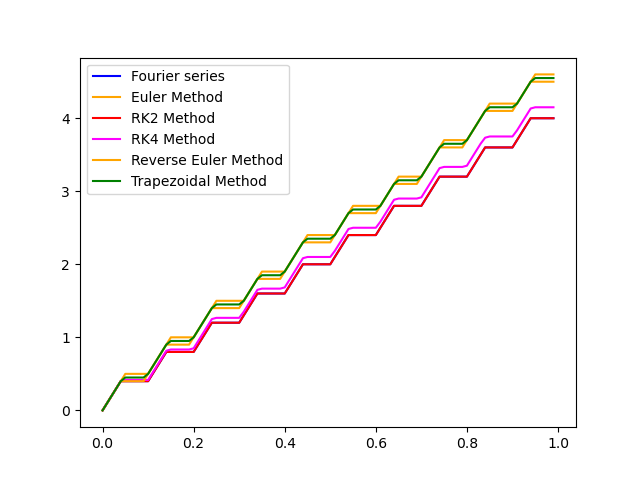
\includegraphics[width=0.45\textwidth]{figs/everything_R0.001_L1_h0.01.png}
    }
    \subfloat[All Methods Error]{
        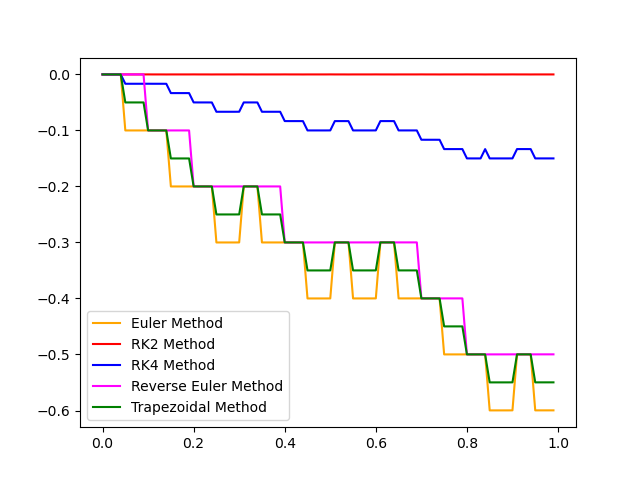
\includegraphics[width=0.45\textwidth]{figs/everythingError_R0.001_L1_h0.01.png}
    }
    \caption{Comparison of All Methods (R = 0.001 $\Omega$, L = 1 H, h = T/10)}
\end{figure}

\subsection{Time Step h = T/1000}

\begin{figure}[H]
    \centering
    \subfloat[Fourier vs Euler]{
        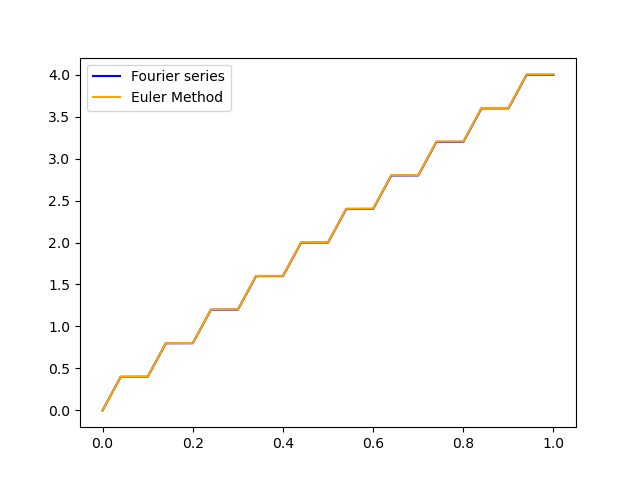
\includegraphics[width=0.45\textwidth]{figs/euler_R0.001_L1_h0.0001.png}
    }
    \subfloat[Euler Error]{
        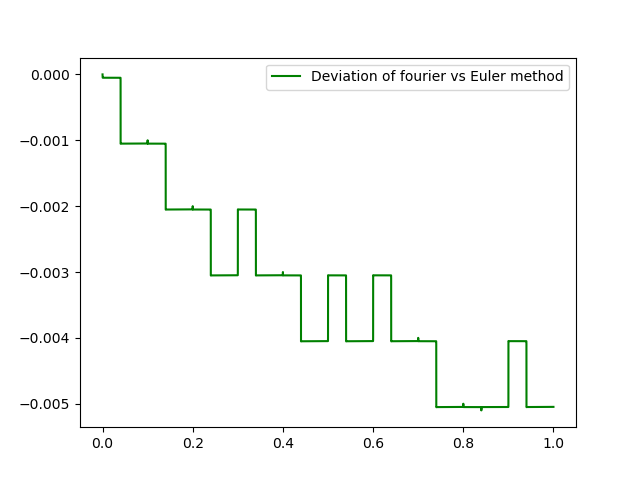
\includegraphics[width=0.45\textwidth]{figs/eulerError_R0.001_L1_h0.0001.png}
    }
    \caption{Euler Method Comparison (R = 0.001 $\Omega$, L = 1 H, h = T/1000)}
\end{figure}

\begin{figure}[H]
    \centering
    \subfloat[Fourier vs RK2]{
        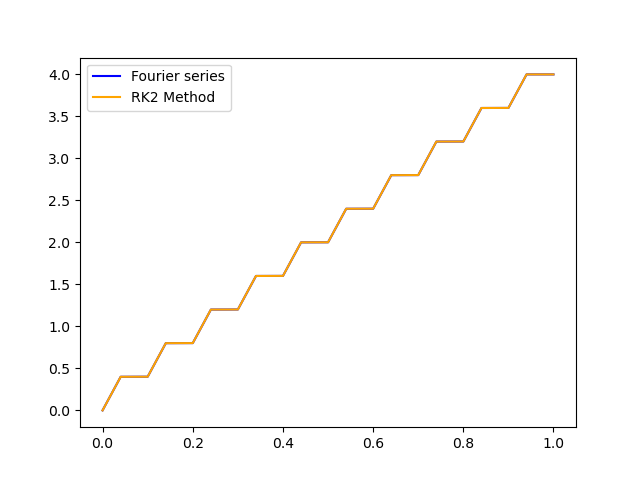
\includegraphics[width=0.45\textwidth]{figs/rk2_R0.001_L1_h0.0001.png}
    }
    \subfloat[RK2 Error]{
        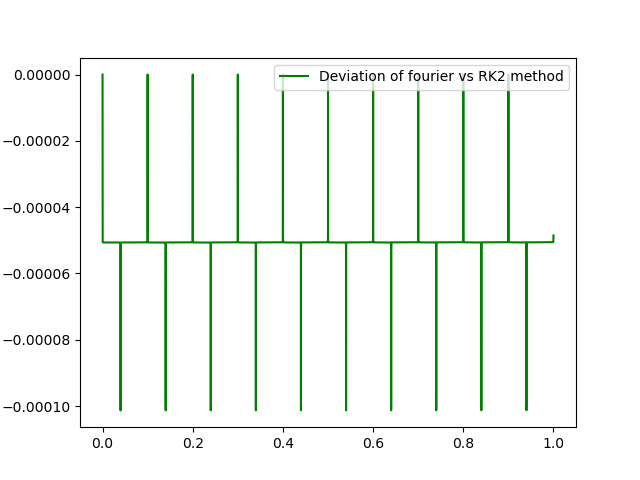
\includegraphics[width=0.45\textwidth]{figs/rk2Error_R0.001_L1_h0.0001.png}
    }
    \caption{RK2 Method Comparison (R = 0.001 $\Omega$, L = 1 H, h = T/1000)}
\end{figure}

\begin{figure}[H]
    \centering
    \subfloat[Fourier vs RK4]{
        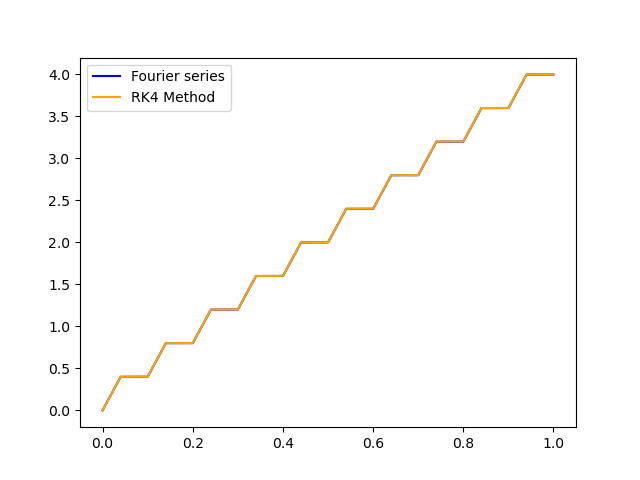
\includegraphics[width=0.45\textwidth]{figs/rk4_R0.001_L1_h0.0001.png}
    }
    \subfloat[RK4 Error]{
        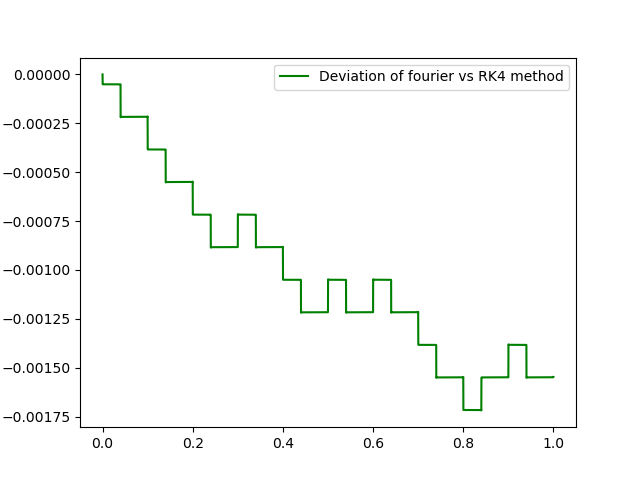
\includegraphics[width=0.45\textwidth]{figs/rk4Error_R0.001_L1_h0.0001.png}
    }
    \caption{RK4 Method Comparison (R = 0.001 $\Omega$, L = 1 H, h = T/1000)}
\end{figure}

\begin{figure}[H]
    \centering
    \subfloat[Fourier vs Reverse Euler]{
        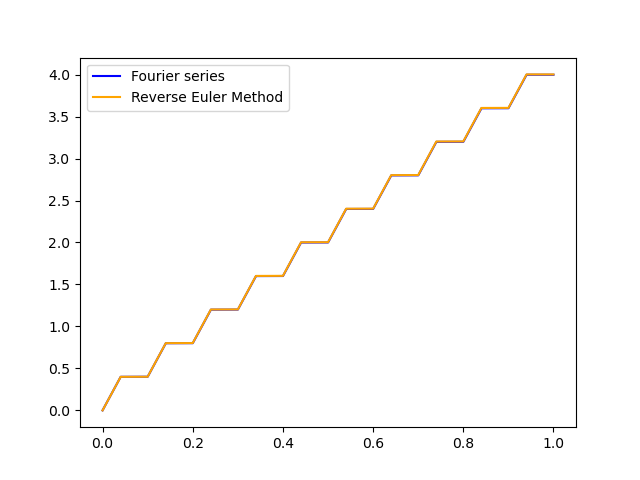
\includegraphics[width=0.45\textwidth]{figs/reverseEuler_R0.001_L1_h0.0001.png}
    }
    \subfloat[Reverse Euler Error]{
        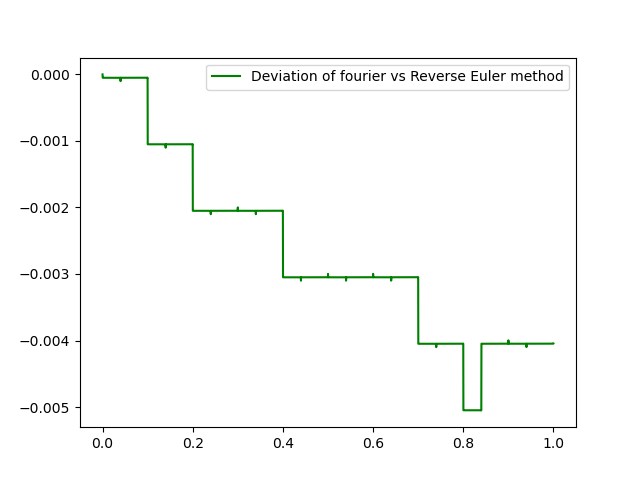
\includegraphics[width=0.45\textwidth]{figs/reverseEulerError_R0.001_L1_h0.0001.png}
    }
    \caption{Reverse Euler Method Comparison (R = 0.001 $\Omega$, L = 1 H, h = T/1000)}
\end{figure}

\begin{figure}[H]
    \centering
    \subfloat[Fourier vs Trapezoidal]{
        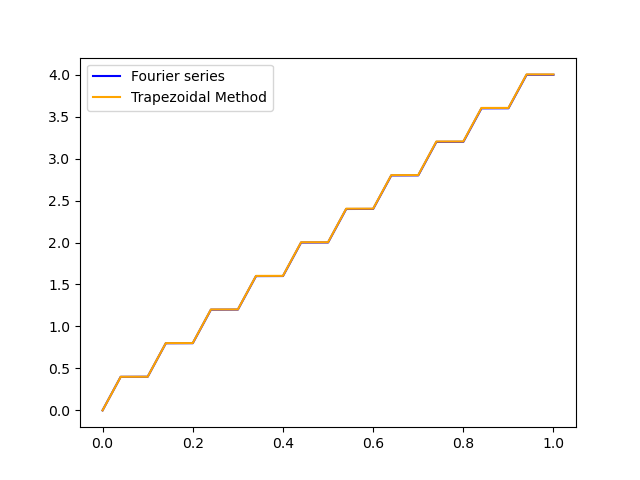
\includegraphics[width=0.45\textwidth]{figs/trapezoidal_R0.001_L1_h0.0001.png}
    }
    \subfloat[Trapezoidal Error]{
        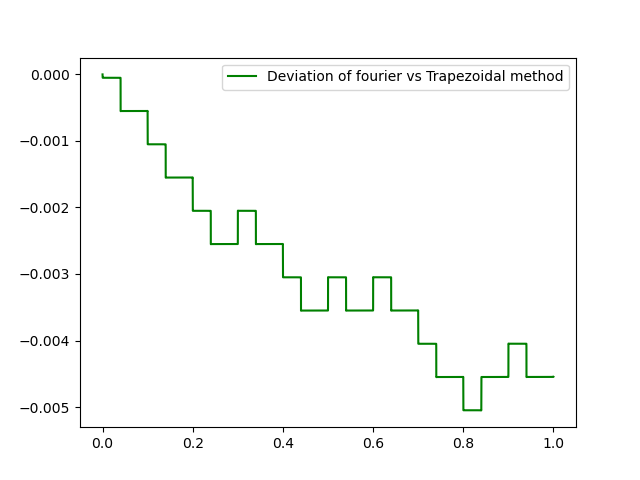
\includegraphics[width=0.45\textwidth]{figs/trapezoidalError_R0.001_L1_h0.0001.png}
    }
    \caption{Trapezoidal Method Comparison (R = 0.001 $\Omega$, L = 1 H, h = T/1000)}
\end{figure}

\begin{figure}[H]
    \centering
    \subfloat[All Methods Comparison]{
        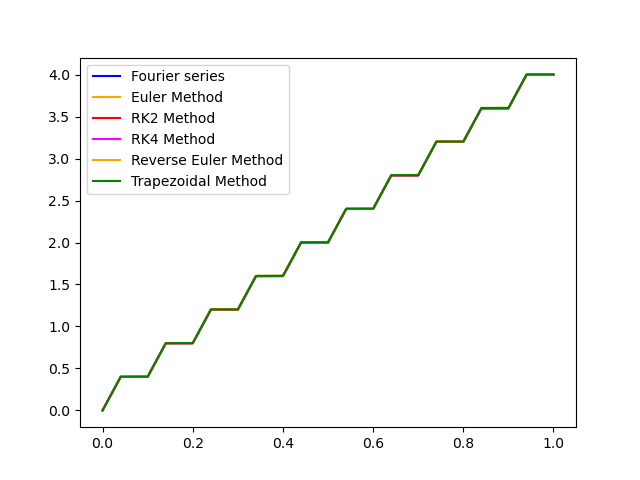
\includegraphics[width=0.45\textwidth]{figs/everything_R0.001_L1_h0.0001.png}
    }
    \subfloat[All Methods Error]{
        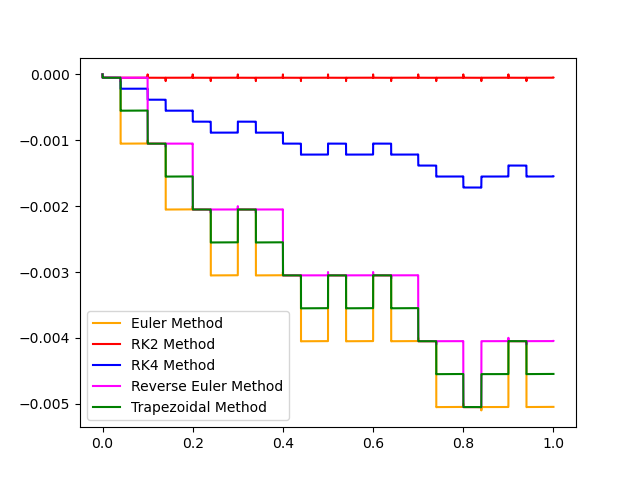
\includegraphics[width=0.45\textwidth]{figs/everythingError_R0.001_L1_h0.0001.png}
    }
    \caption{Comparison of All Methods (R = 0.001 $\Omega$, L = 1 H, h = T/1000)}
\end{figure}

\section{Summary}

This report has presented a comprehensive visual comparison of various numerical methods with the Fourier series solution for an RL circuit with PWM input. The plots show both the direct comparison of current values and the error between each numerical method and the Fourier series solution.

The comparison was conducted across different resistance values (1000 $\Omega$, 100 $\Omega$, 1 $\Omega$, 0.001 $\Omega$) and time steps (T/10, T/1000), while keeping the inductance constant at 1 H. The duty cycle was set at 0.4 and the amplitude at 10.0.

\end{document}
